%%%%%%%%%%%%%%%%%%%%بسمه تعالی%%%%%%%%%%%%%%%%%%%%%%
\documentclass[article]{article}
\usepackage[utf8]{inputenc}
\usepackage{fullpage}

\usepackage[utf8]{inputenc} % allow utf-8 input
\usepackage[T1]{fontenc}    % use 8-bit T1 fonts

\usepackage{booktabs}       % professional-quality tables
\usepackage{amsfonts}       % blackboard math symbols
\usepackage{nicefrac}       % compact symbols for 1/2, etc.
\usepackage{microtype}      % microtypography
\usepackage{amsmath}
\usepackage{tcolorbox}
\definecolor{my-green}{cmyk}{0.2, 0.04, 0.1, 0.04, 0.8}
\usepackage{graphicx}
\usepackage{amsthm}
\usepackage{amssymb}
% \usepackage{cite}
\usepackage[title]{appendix}
\usepackage{algpseudocode}
\usepackage{algorithm}
\usepackage{framed}
\usepackage{mdframed}
\usepackage[pdftex,bookmarks=true,pdfstartview=FitH,colorlinks,linkcolor=magenta,filecolor=blue,citecolor=magenta,urlcolor=blue,pagebackref=false]{hyperref}%
\usepackage{wrapfig}
\usepackage[font=footnotesize,labelsep=space,labelfont=bf]{caption}

\usepackage[top=1in, left=0.9in, right=0.9in, bottom=0.9in]{geometry}
\usepackage{blindtext}
\usepackage{subfigure}
\usepackage{afterpage}
\usepackage{amssymb}% http://ctan.org/pkg/amssymb
\usepackage{pifont}
\usepackage{mathtools}
\DeclarePairedDelimiter{\ceil}{\lceil}{\rceil}
\DeclarePairedDelimiter{\floor}{\lfloor}{\rfloor}
\newcommand{\pl}{Polyak-\L{}ojasiewicz}
\newcommand{\todoM}[1]{\textcolor{blue}{ToDo (Farzin): #1}}
\newcommand{\todo}[1]{\textcolor{red}{ToDo:~#1}}
\newcommand{\alert}[1]{\textcolor{red}{#1}}
\newcommand{\Var}{\mathrm{Var}}
\newcommand{\E}{\mathrm{E}}
\newcommand{\bm}[1]{\boldsymbol{#1}}
\newtheorem{theorem}{Theorem}
\newtheorem{lemma}{Lemma}
\newtheorem{remark}{Remark}
\newtheorem{assumption}{Assumption}
\newtheorem{proposition}{Proposition}
\newtheorem{property}{Property}
\newtheorem{corollary}{Corollary}
\newtheorem{definition}{Definition}
\newtheorem{claim}[theorem]{\bf Claim}
\newtheorem{fact}[theorem]{Fact}
\newtheorem{example}[theorem]{Example}

\newcommand{\belhal}[1]{\todo{{\bf BK:} #1}}

\allowdisplaybreaks

% \input{commands.tex}

\begin{document}

\begin{center}

{\bf{\LARGE{FedSketch: Communication-Efficient and \\
\vspace*{.2in}
Differentially-Private Federated Learning via Sketching}}}
\vspace*{.2in}

{{
%\begin{tabular}{ccc}
%Farzin Haddadpour &
%Weilin Cong & 
%Mehrdad Mahdavi \\ \\
%\end{tabular}
}}
%\begin{tabular}{c}
%School of Electrical Engineering and Computer Science\\
%The Pennsylvania State University\\
%University Park, PA, USA \\
%\texttt{\{fxh18\}@psu.edu}
%\end{tabular}


\vspace*{.2in}



{\large{
\begin{tabular}{c}
%$^\star$
% &  $^\dagger$ 
% & $^{\dagger, \ddagger}$
\end{tabular}
}}
%\vspace*{.2in}

\begin{tabular}{c}
%Microsoft Bing 
%\texttt{Please do not distribute}
%$^\star$
%Department of Electrical Engineering and Computer Sciences, UC Berkeley$^\dagger$ \\
%Department of Statistics, UC Berkeley$^\ddagger$
\end{tabular}

\vspace*{.2in}


\date{\today}

\end{center}

%%%%%%%%%%%%%%%%%%%%%%%%%%%%%%%%%%%%%%%%%%%%%%%%%%%%
\begin{abstract}
Federated learning... 
\end{abstract}
%%%%%%%%%%%%%%%%%%%%%%%%%%%%%%%%%%%%%%%%%%%%%%%%%%%%
\section{Introduction}




%\todo{1) Writing algorithm}





The main contributions of this paper are as follows:
\begin{itemize}
    \item 
\end{itemize}
\todo{Discussing \cite{} One-shot with sketching}




 

%\section{Related Work}



%\section{Gradient Descent based Algorithm and Main Results}

%\subsection{Distributed SGD (Baseline)}

%%%%%%%%%%%%%%%%%%%%%%%%%%%%%%%%%%%%%%%%%%%%%%%%%%%%%%%%
%%%%%%%%%%%%%%%%%%%%%%%%%%%%%%%%%%%%%%%%%%%%%%%%%%%%%%%%
% !TEX root = main.tex
\section{Problem Setting}
In this paper our goal is to solve the following optimization problem using $p$ distributed devices:
\begin{align}
    f(\boldsymbol{x})\triangleq \left[\min_{\boldsymbol{x}\in \mathbb{R}^{d}}\frac{1}{p}\sum_{j=1}^{p}F_j(\boldsymbol{x})\right]
\end{align}
where $F_j(\boldsymbol{x})=\mathbb{E}_{\xi\in\mathcal{D}_j}\left[f_j\left(\boldsymbol{x},\xi\right)\right]$ is the local cost function at device $j$. $\xi$ is a random variable with probability distribution $\mathcal{D}_j$.

\todo{Differences and potential improvements over \cite{haddadpour2020federated}!}


\section{Count Sketch Review}

%%%%%%%%%%%%%%%%%%%%%%%%%%%%%%%%%%%%%%
%%%%%%%%%%%%%%%%%%%%%%%%%%%%%%%%%%%%%%%
\begin{algorithm}[H]
\caption{\texttt{CS}: Count Sketch to compress ${\boldsymbol{x}}\in\mathbb{R}^{d}$. }\label{Alg:csketch}
\begin{algorithmic}[1]
\State \textbf{Inputs:} $\boldsymbol{x}\in\mathbb{R}^{d}, t, k, \mathbf{S}_{t\times k}, h_i (1\leq i\leq t), sign_i (1\leq i\leq t)$
\State \textbf{Compress vector $\boldsymbol{x}\in\mathbb{R}^{d}$ into $\mathbf{S}\left(\boldsymbol{x}\right)$:}
\State \textbf{for} $\boldsymbol{x}_i\in\boldsymbol{x}$ \textbf{do}
\State \quad\textbf{for $j=1,\cdots,t$ do}
\State \quad\quad $\mathbf{S}[j][h_j(i)]=\mathbf{S}[j-1][h_{j-1}(i)]+\text{sign}_j(i).\boldsymbol{x}_i$ 
\State \quad\textbf{end for}
\State \textbf{end for}
\State \textbf{return} $\mathbf{S}_{t\times k}(\boldsymbol{x})$
\end{algorithmic}
\end{algorithm}
%%%%%%%%%%%%%%%%%%%%%%%%%%%%%%%%%%%%%%%%%%
%We indicate the total size of the sketch with $D$.
\paragraph{Notation:} For the rest of the paper we indicate the number of communication rounds and number of bits per round per device with $R(\epsilon)$ and $B(d)$ respectively. For the rest of the paper we indicate the count sketch of any vector $\boldsymbol{x}$ with $\mathbf{S}(\boldsymbol{x})$
\section{Compression Operations}
In this subsection, we review a recent results that will be useful for our work. Similar to \cite{horvath2020better}, we define the following two types of compressor operators that will be useful for our algorithm.
\subsection{Unbiased Compressor}
\begin{definition}[Unbiased compressor]
A randomized function, $\text{C}:\mathbb{R}^{d}\rightarrow\mathbb{R}^{d}$ is called an unbiased compression operator with $\Delta\geq 1$, if we have 
\begin{align}
\mathbb{E}\left[\text{C}(\boldsymbol{x})\right]&=\boldsymbol{x}\nonumber\\
    \mathbb{E}\left[\left\|\text{C}(\boldsymbol{x})\right\|^2_2\right]&\leq \Delta\left\|\boldsymbol{x}\right\|^2_2
\end{align}
We indicate this class of compressor with $\text{C}\in\mathbb{U}(\Delta)$
\end{definition}
We note that this definition leads to the property 
\begin{align}
    \mathbb{E}\left[\left\|\text{C}(\boldsymbol{x})-\boldsymbol{x}\right\|^2_2\right]&\leq \left(\Delta-1\right)\left\|\boldsymbol{x}\right\|^2_2
\end{align}
\begin{remark}
Note that in case of $\Delta=1$ our algorithm reduces for the case of no compression. This property allows us the noise of the compression.
\end{remark}
%%%%%%%%%%%%%%%%%%%%%%%%%%%%%%%%%%%%%%
%%%%%%%%%%%%%%%%%%%%%%%%%%%%%%%%%%%%%%%
\begin{algorithm}[H]
\caption{\texttt{PRIVIX}\cite{li2019privacy}: Unbiased compressor based on sketching. }\label{Alg:csketch}
\begin{algorithmic}[1]
\State \textbf{Inputs:} $\boldsymbol{x}\in\mathbb{R}^{d}, t, k, \mathbf{S}_{t\times k}, h_i (1\leq i\leq t), sign_i (1\leq i\leq t)$
%\State \textbf{Compress vector $\tilde{\mathbf{g}}\in\mathbb{R}^{d}$ into $\mathbf{S}\left(\tilde{\mathbf{g}}\right)$:}
%\State \textbf{for} $\mathbf{g}_i\in\mathbf{g}$ \textbf{do}
%\State \quad\textbf{for $j=1,\cdots,t$ do}
%\State \quad\quad $\mathbf{S}[j][h_j(i)]=\mathbf{S}[j-1][h_{j-1}(i)]+\text{sign}_j(i).\mathbf{g}_i$ 
%\State \quad\textbf{end for}
%\State \textbf{end for}
%\State \textbf{return} $\mathbf{S}_{t\times k}$
\State \textbf{Query} $\tilde{\boldsymbol{x}}\in\mathbb{R}^d$ \textbf{from $\mathbf{S(\boldsymbol{x})}$:}
\State \textbf{for} $i=1,\ldots,d$ \textbf{do}
\State \quad\quad ${\tilde{\boldsymbol{x}}}[i]=\text{Median}\{\text{sign}_j(i).\mathbf{S}[j][h_j(i)]:1\leq j\leq t\}$ 
\State \textbf{end for}
\State \textbf{Output:} ${\tilde{\boldsymbol{x}}}$
%\belhal{What is this function $\mathbf{S}(\cdot)$?. Do you mean the matrix $\mathbf{S}_g$ ? }
%\textcolor{blue}{Farzin: I will change the notation later, see \cite{li2019privacy} for the original algorithm!}
\vspace{- 0.1cm}
\end{algorithmic}
\end{algorithm}
%%%%%%%%%%%%%%%%%%%%%%%%%%%%%%%%%%%%%%%%%%
\paragraph{Estimation errors:}

\begin{property}[\cite{li2019privacy}]
For our proof purpose we will need the following crucial properties of the count sketch described in Algorithm~\ref{Alg:csketch}, for any real valued vector $\mathbf{x}\in \mathbb{R}^{d}$:
\begin{itemize}
    \item[1)] \emph{Unbiased estimation}: As it is also mentioned in \cite{li2019privacy}, we have:
    \begin{align}
        \mathbb{E}_{\mathbf{S}}\left[\texttt{PRIVIX}\left[\mathbf{S}\left(\mathbf{x}\right)\right]\right]=\mathbf{x}
    \end{align}
    %\belhal{The biased case is interesting, no hopes dealing with it for now?}
    
    %\textcolor{blue}{Farzin: See Algorithms 5 and 6, yet I am working on the convergence proof! Plus, this is the property of the count sketch not assumption, so I think we are good even for unbiased case!}
    \item[2)] \emph{Bounded variance}: With $k=O\left(\frac{e}{\mu^2}\right)$ and $t=O\left(\ln \left(\frac{1}{\delta}\right)\right)$, we have the following bound with probability $1-\delta$:
    \begin{align}
        \mathbb{E}_{\mathbf{S}}\left[\left\|\texttt{PRIVIX}\left[\mathbf{S}\left(\mathbf{x}\right)\right]-\mathbf{x}\right\|_2^2\right]\leq \mu^2 d\left\|\mathbf{x}\right\|_2^2
    \end{align}
\end{itemize}
\end{property}
Therefore, $\texttt{PRIVIX}\in \mathbb{U}(1+\mu^2 d)$ with probability $1-\delta$.
\begin{remark}
We note that $\Delta=1+\mu^2d$ implies that if $k\rightarrow d$, $\Delta\rightarrow 1+1=2$, which means that the case of no compression is not covered. Thus, the algorithms based on this may converges poorly.
\end{remark}

\paragraph{Differentially Private Property:}
\begin{definition}
A randomized mechanism $\mathcal{O}$ satisfies $\epsilon-$differential privacy, if for input data ${S}_1$ and ${S}_2$ differing by up to one element, and for any output $D$ of $\mathcal{O}$,
\begin{align}
    \Pr\left[\mathcal{O}(S_1)\in D\right]\leq \exp{\left(\epsilon\right)}\Pr\left[\mathcal{O}(S_2)\in D\right] 
\end{align}
\end{definition}
\todo{Add explanations that this scheme induces local privacy!}

\begin{assumption}[Input vector distribution]\label{assu:invecdist}
For the purpose of privacy analysis, similar to \cite{,}, we suppose that for any input vector $S$ with length $|S|=l$, each element $s_i\in S$ is drawn i.i.d. from a Gaussian distribution: $s_i\sim \mathcal{N}(0,\sigma^2)$, and bounded by a large probability:  $|s_i|\leq C, 1\leq i\leq p$ for some positive constant $C>0$.    
\end{assumption}

\begin{theorem}[$\epsilon-$ differential privacy of count sketch, \cite{li2019privacy}]
For a sketching algorithm $\mathcal{O}$ using Count Sketch $\mathbf{S}_{t\times k}$ with $t$ arrays of $k$ bins, for any input vector $S$ with length $l$ satisfying Assumption~\ref{assu:invecdist}, $\mathcal{O}$ achieves $t.\ln \left(1+\frac{\alpha C^2 k(k-1)}{\sigma^2(l-2)}(1+\ln(l-k) )\right)-$differential privacy with high probability, where $\alpha$ is a positive constant satisfying $\frac{\alpha C^2 k(k-1)}{\sigma^2(l-2)}(1+\ln(l-k) )\leq \frac{1}{2}-\frac{1}{\alpha}$.
\end{theorem}
The proof of this theorem can be found in \cite{li2019privacy}.




\subsection{Biased compressor}
\begin{definition}[Biased compressor]
A (randomized) function,  ${\text{C}}:\mathbb{R}^{d}\rightarrow\mathbb{R}^{d}$ is called a compression operator with $\alpha>0$ and $\Delta\geq 1$, if we have 
\begin{align}
    \mathbb{E}\left[\left\|\alpha\boldsymbol{x}-\bar{\text{C}}(\boldsymbol{x})\right\|^2_2\right]\leq \left(1-\frac{1}{\Delta}\right)\left\|\boldsymbol{x}\right\|^2_2
\end{align}
Any biased compression operator $C$ is indicated by $C\in \mathbb{C}(\Delta,\alpha)$. 
\end{definition}
The following Lemma links these two definitions:
\begin{lemma}[\cite{horvath2020better}]
We have $\mathbb{U}(\Delta)\subset\mathbb{C}(\Delta)$.
\end{lemma}

An instance of biased compressor based on sketching is as follows:
%%%%%%%%%%%%%%%%%%%%%%%%%%%%%%%%%%
\begin{algorithm}[H]
\caption{\texttt{HEAVYMIX}~\cite{ivkin2019communication} }\label{Alg:sketch}
\begin{algorithmic}[1]
\State \textbf{Inputs:} $\mathbf{S}_{\mathbf{g}}$; parameter-$k$
\State \textbf{Compress vector $\tilde{\mathbf{g}}\in\mathbb{R}^{d}$ into $\mathbf{S}\left(\tilde{\mathbf{g}}\right)$:}
\State Query $\hat{\ell}_2^2=\left(1\pm 0.5\right)\left\|\mathbf{g}\right\|^2$ from sketch $\mathbf{S}_{\mathbf{g}}$
\State $\forall j$ query $\hat{\mathbf{g}}_j^2=\hat{\mathbf{g}}_j^2\pm \frac{1}{2k}\left\|\mathbf{g}\right\|^2$ from sketch $\mathbf{S}_{\mathbf{g}}$
\State $H=\{j|\hat{\mathbf{g}}_j\geq \frac{\hat{\ell}_2^2}{k}\}$ and $NH=\{j|\hat{\mathbf{g}}_j<\frac{\hat{\ell}_2^2}{k}\}$
\State Top$_k=H\cup rand_\ell(NH)$, where $\ell=k-\left|H\right|$
\State Get exact values of Top$_k$ 
\State \textbf{Output:} $\mathbf{g}_S:\forall j\in\text{Top}_k:\mathbf{g}_{Si}=\mathbf{g}_{i}$ and $\forall\notin\text{Top}_k: \mathbf{g}_{Si}=0$
%\vspace{- 0.1cm}
\end{algorithmic}
\end{algorithm}
%%%%%%%%%%%%%%%%%%%%%%%%%%%%%%%%%%%%%%%%%%
\todo{Explain minor distinction here!}

\begin{lemma}[\cite{ivkin2019communication}]
\texttt{HEAVYMIX}, with sketch size $\Theta\left(k\log\left(\frac{d}{\delta}\right)\right)$ is a biased compressor with $\alpha=1$ and  $\Delta=d/k$ with probability $\geq1-\delta$. In other words, with probability $1-\delta$, $\texttt{HEAVYMIX}\in C(\frac{d}{k},1)$. 
\end{lemma}
\subsection{Sketching Based on Induced Compressor}
The following Lemma from~\cite{horvath2020better} shows that how we can transfer biased compressor into an unbiased compressor: 
\begin{lemma}[Induced Compressor ~\cite{horvath2020better}]\label{lemm:induced_compress}
For $C_1\in \mathbb{C}(\Delta_1)$ with $\alpha=1$, choose $C_2\in \mathbb{U}(\Delta_2)$ and define the induced compressor with
\begin{align}
    C(\mathbf{x})=C_1(\mathbf{x})+C_2\left(x-C_1\left(\mathbf{x}\right)\right)
\end{align}
The induced compressor $C$ satisfies $C\in\mathbb{U}(\mathbf{x})$ with $\Delta=\Delta_2+\frac{1-\Delta_2}{\Delta_1}$.
\end{lemma}
\begin{remark}
We note that if $\Delta_2\geq 1$ and $\Delta_1\leq 1$, we have $\Delta=\Delta_2+\frac{1-\Delta_2}{\Delta_1}\leq \Delta_2$
\end{remark}
Using this concept of the induced compressor we introduce the following:


\begin{corollary}
Based on Lemma~\ref{lemm:induced_compress} and defining 
\begin{align}
    \texttt{HEAPRIX}\left[\mathbf{S}\left(\boldsymbol{x}\right)\right]=\texttt{HEAVYMIX}\left[\mathbf{S}\left(\mathbf{x}\right)\right]+\texttt{PRIVIX}\left[\mathbf{S}\left(\mathbf{x}-\texttt{HEAVYMIX}\left[\mathbf{S}\left(\mathbf{x}\right)\right]\right)\right]
\end{align}

we have $C(x)\in \mathbb{U}(\mu^2 d)$.
\end{corollary}
\begin{remark}
We highlight that in this case if $k\rightarrow d$, then $C(x)\rightarrow x$ which means that your convergence algorithm can be improved by decreasing the noise of compression (with choice of bigger $k$). 
\end{remark}

%%%%%%%%%%%%%%%%%%%%%%%%%%%%%%%%%%%%%
%%%%%%%%%%%%%%%%%%%%%%%%%%%%%%%%%%%%%
In the following we define two general framework for different sketching algorithms for homogeneous and heterogeneous data distributions.
\section{Algorithms for homogeneous and heterogeneous settings}
In the following, first we present two algorithm for homogeneous setting. Then, we present two algorithms for heterogeneous algorithms to deal with data heterogeneity.   

\subsection{Homogeneous setting}
In this section, we propose two algorithms for the setting where data at distributed devices is  correlated. The proposed Federated Learning with averaging uses sketching to compress communication. The main difference between first algorithm and the algorithm in \cite{li2019privacy} is that we use distinct local and global learning rates. Additionally, unlike \cite{li2019privacy} we do not add add local Gaussian noise for the privacy purpose. 

In \texttt{FedSKETCH-I}, we indicate the number of communication rounds between devices and server with $R$, and the number of local updates at device $j$ is illustrated with $\tau$, which happens between two consecutive communication rounds. Unlike \cite{haddadpour2020federated}, server node does not store any global model, instead device $j$ has two models, $\boldsymbol{x}^{(r)}$ and $\boldsymbol{x}^{(\ell,r)}_j$. In communication round $r$ device $j$, the local model $\boldsymbol{x}^{(\ell,r)}_j$ is updated using the rule $$\boldsymbol{x}_j^{(\ell+1,r)}=\boldsymbol{x}_j^{(\ell,r)}-\eta \tilde{\mathbf{g}}_j^{(\ell,r)}, \qquad\qquad \text{for}\:\:\ell=0,\ldots,\tau-1$$
where $\tilde{\mathbf{g}}_j^{(\ell,r)}\triangleq\nabla{f}_j(\boldsymbol{x}_j^{(\ell,r)},\Xi_j^{(\ell,r)})\triangleq\frac{1}{b}\sum_{\xi\in\Xi_j^{(\ell,r)}}\nabla{L}_j(\boldsymbol{x}_j^{(\ell,r)},\xi)$ is a stochastic gradient of $f_j$ evaluated using the mini-batch $\Xi_j^{(\ell,r)}=\{\xi^{(\ell,r)}_{j,1},\ldots,\xi^{(\ell,r)}_{j,b_j} \}$ of size $b_j$. $\eta$ is the local learning rate. After $\tau$ local updates locally, model at device $j$ and communication round $r$ is indicated by $\boldsymbol{x}_j^{(\tau,r)}$. The next step of our algorithm is that device $j$ sends the count sketch $\mathbf{S}_j^{(r)}\triangleq\mathbf{S}_j\left(\boldsymbol{x}_j^{(\tau,r)}-\boldsymbol{x}_j^{(0,r)}\right)$ back to the server. We highlight that $$\mathbf{S}_j^{(r)}\triangleq\mathbf{S}_j\left(\boldsymbol{x}_j^{(\tau,r)}-\boldsymbol{x}_j^{(0,r)}\right)=\mathbf{S}_j\left(\eta\sum_{\ell=0}^{\tau-1}\tilde{\mathbf{g}}_j^{(\ell,r)}\right)=\eta\mathbf{S}_j\left(\sum_{\ell=0}^{\tau-1}\tilde{\mathbf{g}}_j^{(\ell,r)}\right),$$ which is the aggregation of the consecutive stochastic gradients multiplied with local updates $\eta$.

Upon receiving all $\mathbf{S}_j^{(r)}$ from devices, the server computes 
\begin{align}
    \mathbf{S}^{(r)}=\frac{1}{p}\sum_{j=1}^p\mathbf{S}_j^{(r)}
\end{align}
and broadcasts it to all devices. Devices after receiving $\mathbf{S}^{(r)}$ from server updates  global model $\boldsymbol{x}^{(r)}$ using rule $$\boldsymbol{x}^{(r)}=\boldsymbol{x}^{(r-1)}-\gamma \texttt{PRIVIX}\left[\mathbf{S}^{(r-1)}\right]$$
All these steps are summarized in \texttt{FedSKETCH-I} (Algorithm~\ref{Alg:PFLHom-I}).
\begin{algorithm}[H]
\caption{\texttt{FedSKETCH-I}($R$, $\tau, \eta, \gamma$): Private Federated Learning with Sketching. }\label{Alg:PFLHom-I}
\begin{algorithmic}[1]
\State \textbf{Inputs:} $\boldsymbol{x}^{(0)}$ as an initial  model shared by all local devices, the number of communication rounds $R$, the the number of local updates $\tau$, and global and local learning rates $\gamma$ and $\eta$, respectively
%\State Server chooses a subset $\mathcal{P}_0$ of $K$ devices at random (device $j$ is chosen with probability $q_j$);
\State \textbf{for $r=0, \ldots, R-1$ do}
\State $\qquad$\textbf{parallel for device $j=1,\ldots,n$ do}:
\State $\qquad\quad$ Set $\boldsymbol{x}^{(r)}=\boldsymbol{x}^{(r-1)}-\gamma{\texttt{PRIVIX}}\left[{\mathbf{S}}^{(r-1)}\right]$ 
\State $\qquad\quad$ Set $\boldsymbol{x}_j^{(0,r)}=\boldsymbol{x}^{(r)}$ 
\State $\qquad\quad $\textbf{for} $c=0,\ldots,\tau-1$ \textbf{do}
\State $\qquad\quad\quad$ Sample a mini-batch $\xi_j^{(\ell,r)}$ and compute $\tilde{\mathbf{g}}_{j}^{(\ell,r)}\triangleq\nabla{f}_j(\boldsymbol{x}^{(\ell,r)}_j,\xi_j^{(c,r)})$
\State $\qquad\quad\quad$ $\boldsymbol{x}^{(\ell+1,r)}_{j}=\boldsymbol{x}^{(\ell,r)}_j-\eta~ \tilde{\mathbf{g}}_{j}^{(\ell,r)}$ \label{eq:update-rule-alg}
\State $\qquad\quad$\textbf{end for}
\State $\qquad\quad\quad$Device $j$ sends $\mathbf{S}^{(r)}_{j}\triangleq\mathbf{S}_{j}\left(\boldsymbol{x}_j^{(0,r)}-~{\boldsymbol{x}}_{j}^{(\tau,r)}\right)$ back to the server.
\State $\qquad$Server \textbf{computes} 
\State $\qquad\qquad {\mathbf{S}}^{(r)}=\frac{1}{p}\sum_{j=1}\mathbf{S}^{(r)}_{j}$ and \textbf{broadcasts} ${\mathbf{S}}^{(r)}$ to all devices.
%\State $\qquad$Sever chooses a set of devices  $\mathcal{P}_t$ with distribution $q_j$.
%\State $\qquad\quad$ \textbf{end if}
\State $\qquad$\textbf{end parallel for}
\State \textbf{end}
\State \textbf{Output:} ${\boldsymbol{x}}^{(R-1)}$
\vspace{- 0.1cm}
%\State \todo{How about we call the algorithm local SGD with decoupled rates (LSDR) and specialize the analysis for IID and non-IID cases}
\end{algorithmic}
\end{algorithm}
%%%%%%%%%%%%%%%%%%%%%%%%%%%%%%%%%%%%%%%%%%

Next, we describe our algorithm using induced sketching.






\begin{algorithm}[H]
\caption{\texttt{FedSKETCH-II}($R$, $\tau, \eta, \gamma$): Private Federated Learning with Sketching. }\label{Alg:PFLHom}
\begin{algorithmic}[1]
\State \textbf{Inputs:} $\boldsymbol{x}^{(0)}$ as an initial  model shared by all local devices, the number of communication rounds $R$, the the number of local updates $\tau$, and global and local learning rates $\gamma$ and $\eta$, respectively
%\State Server chooses a subset $\mathcal{P}_0$ of $K$ devices at random (device $j$ is chosen with probability $q_j$);
\State \textbf{for $r=0, \ldots, R-1$ do}

\State $\qquad$\textbf{parallel for device $j=1,\ldots,n$ do}:
\State $\qquad\quad$ Computes ${\mathbf{\Phi}}^{(r-1)}\triangleq \texttt{HEAVYMIX}(\mathbf{S}^{(r-1)})+\texttt{PRIVIX}\left[{\mathbf{S}}^{(r-1)}- \tilde{\mathbf{S}}^{(r-1)}\right]$


\State $\qquad\quad$ Set $\boldsymbol{x}^{(r)}=\boldsymbol{x}^{(r-1)}-\gamma{\mathbf{\Phi}}^{(r-1)}$
\State $\qquad\quad$ Set $\boldsymbol{x}_j^{(0,r)}=\boldsymbol{x}^{(r)}$ 
\State $\qquad\quad $\textbf{for} $c=0,\ldots,\tau-1$ \textbf{do}
\State $\qquad\quad\quad$ Sample a mini-batch $\xi_j^{(\ell,r)}$ and compute $\tilde{\mathbf{g}}_{j}^{(\ell,r)}\triangleq\nabla{f}_j(\boldsymbol{x}^{(\ell,r)}_j,\xi_j^{(c,r)})$
\State $\qquad\quad\quad$ $\boldsymbol{x}^{(\ell+1,r)}_{j}=\boldsymbol{x}^{(\ell,r)}_j-\eta~ \tilde{\mathbf{g}}_{j}^{(c,r)}$ \label{eq:update-rule-alg}
\State $\qquad\quad$\textbf{end for}
\State $\qquad\quad\quad$Device $j$ sends $\mathbf{S}^{(r)}_{j}\triangleq\mathbf{S}_{j}\left(\boldsymbol{x}_j^{(0,r)}-~{\boldsymbol{x}}_{j}^{(\tau,r)}\right)$ back to the server.
\State $\qquad$Server \textbf{computes} 
\State $\qquad\qquad {\mathbf{S}}^{(r)}=\frac{1}{p}\sum_{j=1}\mathbf{S}^{(r)}_{j}$ and \textbf{broadcasts} ${\mathbf{S}}^{(r)}$ to all devices.
\State $\qquad$ Second round of communication to obtain $\delta_j^{(r)} :=  \mathbf{S}_j\left[\texttt{HEAVYMIX}(\mathbf{S}^{(r)})\right]$ 
\State $\qquad$ Broadcasts $\tilde{\mathbf{S}}^{(r)}\triangleq\frac{1}{p}\sum_{j=1}^p\delta_j^{(r)}$ to devices
\State $\qquad$\textbf{end parallel for}
\State \textbf{end}
\State \textbf{Output:} ${\boldsymbol{x}}^{(R-1)}$
\vspace{- 0.1cm}
%\State \todo{How about we call the algorithm local SGD with decoupled rates (LSDR) and specialize the analysis for IID and non-IID cases}
\end{algorithmic}
\end{algorithm}


\todo{revise it!}

%%%%%%%%%%%%%%%%%%%%%%%%%%%%%%%%%%%%%%%%%%




\subsection{Heterogeneous setting}

\begin{algorithm}[H]
\caption{\texttt{FedSKETCHGATE-I}($R$, $\tau, \eta, \gamma$): Private Federated Learning with Sketching and gradient tracking. }\label{Alg:PFLHet}
\begin{algorithmic}[1]
\State \textbf{Inputs:} $\boldsymbol{x}^{(0)}=\boldsymbol{x}^{(0)}_j$ as an initial  model shared by all local devices, the number of communication rounds $R$, the the number of local updates $\tau$, and global and local learning rates $\gamma$ and $\eta$, respectively
%\State Server chooses a subset $\mathcal{P}_0$ of $K$ devices at random (device $j$ is chosen with probability $q_j$);
\State \textbf{for $r=0, \ldots, R-1$ do}
\State $\qquad$\textbf{parallel for device $j=1,\ldots,n$ do}:
\State $\qquad\quad$ Set $\mathbf{c}_j^{(r)}=\mathbf{c}_j^{(r-1)}-\frac{1}{\tau}\left({\texttt{PRIVIX}}\left(\mathbf{S}^{(r-1)}\right)-{\texttt{PRIVIX}}\left(\mathbf{S}^{(r-1)}_{j}\right)\right)$
\State $\qquad\quad$ Set $\boldsymbol{x}^{(r)}=\boldsymbol{x}^{(r-1)}-\gamma{\texttt{PRIVIX}}\left(\mathbf{S}^{(r-1)}\right)$
\State $\qquad\quad$ Set $\boldsymbol{x}_j^{(0,r)}=\boldsymbol{x}^{(r)}$ % \belhal{Where do we compute/define $\boldsymbol{x}^{(r-1)}$ ?}\textcolor{blue}{FH: Added to previous line!}
\State $\qquad\quad $\textbf{for} $\ell=0,\ldots,\tau-1$ \textbf{do}
\State $\qquad\quad\quad$ Sample a mini-batch $\xi_j^{(\ell,r)}$ and compute $\tilde{\mathbf{g}}_{j}^{(\ell,r)}\triangleq\nabla{f}_j(\boldsymbol{x}^{(\ell,r)}_j,\xi_j^{(\ell,r)})$
\State $\qquad\quad\quad$ $\boldsymbol{x}^{(\ell+1,r)}_{j}=\boldsymbol{x}^{(\ell,r)}_j-\eta~\left( \tilde{\mathbf{g}}_{j}^{(\ell,r)}-\mathbf{c}_j^{(r)}\right)$ \label{eq:update-rule-alg}
\State $\qquad\quad$\textbf{end for}
\State $\qquad\quad\quad$Device $j$ sends $\mathbf{S}^{(r)}_{j}\triangleq\mathbf{S}\left(\boldsymbol{x}_j^{(0,r)}-~{\boldsymbol{x}}_{j}^{(\tau,r)}\right)$ back to the server.
\State $\qquad$Server \textbf{computes} 
\State $\qquad\qquad {\mathbf{S}}^{(r)}=\frac{1}{p}\sum_{j=1}\mathbf{S}^{(r)}_{j}$ and  \textbf{broadcasts} ${\mathbf{S}}^{(r)}$ to all devices.
%\State $\qquad$Sever chooses a set of devices  $\mathcal{P}_t$ with distribution $q_j$.
%\State $\qquad\quad$ \textbf{end if}
\State $\qquad$\textbf{end parallel for}
\State \textbf{end}
\State \textbf{Output:} ${\boldsymbol{x}}^{(R-1)}$
\vspace{- 0.1cm}
%\State \todo{How about we call the algorithm local SGD with decoupled rates (LSDR) and specialize the analysis for IID and non-IID cases}
\end{algorithmic}
\end{algorithm}


\todo{revise it!}

\begin{algorithm}[H]
\caption{\texttt{FedSKETCHGATE-II}($R$, $\tau, \eta, \gamma$): Private Federated Learning with Sketching and gradient tracking. }\label{Alg:PFLHet}
\begin{algorithmic}[1]
\State \textbf{Inputs:} $\boldsymbol{x}^{(0)}=\boldsymbol{x}^{(0)}_j$ as an initial  model shared by all local devices, the number of communication rounds $R$, the the number of local updates $\tau$, and global and local learning rates $\gamma$ and $\eta$, respectively
%\State Server chooses a subset $\mathcal{P}_0$ of $K$ devices at random (device $j$ is chosen with probability $q_j$);
\State \textbf{for $r=0, \ldots, R-1$ do}
\State $\qquad$\textbf{parallel for device $j=1,\ldots,n$ do}:
\State $\qquad\quad$ Computes ${\mathbf{\Phi}}(\mathbf{S}^{(r-1)})\triangleq \texttt{HEAVYMIX}(\mathbf{S}^{(r-1)})+\texttt{PRIVIX}\left[{\mathbf{S}}^{(r-1)}- \tilde{\mathbf{S}}^{(r-1)}\right]$
\State $\qquad\quad$ Set $\mathbf{c}_j^{(r)}=\mathbf{c}_j^{(r-1)}-\frac{1}{\tau}\left(\mathbf{\Phi}\left(\mathbf{S}^{(r-1)}\right)-\mathbf{\Phi}\left(\mathbf{S}^{(r-1)}_{j}\right)\right)$
\State $\qquad\quad$ Set $\boldsymbol{x}^{(r)}=\boldsymbol{x}^{(r-1)}-\gamma\mathbf{\Phi}\left(\mathbf{S}^{(r-1)}\right)$
\State $\qquad\quad$ Set $\boldsymbol{x}_j^{(0,r)}=\boldsymbol{x}^{(r)}$ % \belhal{Where do we compute/define $\boldsymbol{x}^{(r-1)}$ ?}\textcolor{blue}{FH: Added to previous line!}
\State $\qquad\quad $\textbf{for} $\ell=0,\ldots,\tau-1$ \textbf{do}
\State $\qquad\quad\quad$ Sample a mini-batch $\xi_j^{(\ell,r)}$ and compute $\tilde{\mathbf{g}}_{j}^{(\ell,r)}\triangleq\nabla{f}_j(\boldsymbol{x}^{(\ell,r)}_j,\xi_j^{(\ell,r)})$
\State $\qquad\quad\quad$ $\boldsymbol{x}^{(\ell+1,r)}_{j}=\boldsymbol{x}^{(\ell,r)}_j-\eta~\left( \tilde{\mathbf{g}}_{j}^{(\ell,r)}-\mathbf{c}_j^{(r)}\right)$ \label{eq:update-rule-alg}
\State $\qquad\quad$\textbf{end for}
\State $\qquad\quad\quad$Device $j$ sends $\mathbf{S}^{(r)}_{j}\triangleq\mathbf{S}\left(\boldsymbol{x}_j^{(0,r)}-~{\boldsymbol{x}}_{j}^{(\tau,r)}\right)$ back to the server.
\State $\qquad\quad\quad$Device $j$ computes $$\mathbf{\Phi}\left(\mathbf{S}^{(r)}_{j}\right)\triangleq \texttt{HEAVYMIX}[\mathbf{S}_j^{(r)}]+\texttt{PRIVIX}\left[{\mathbf{S}}_j^{(r)}- {\mathbf{S}_j}^{(r)}\left(\texttt{HEAVYMIX}[{\mathbf{S}_j}^{(r)}]\right)\right]$$
\State $\qquad$Server \textbf{computes} 
\State $\qquad\qquad {\mathbf{S}}^{(r)}=\frac{1}{p}\sum_{j=1}\mathbf{S}^{(r)}_{j}$ and  \textbf{broadcasts} ${\mathbf{S}}^{(r)}$ to all devices.
\State $\qquad$ Second round of communication to obtain $\delta_j^{(r)} :=  \mathbf{S}_j\left(\texttt{HEAVYMIX}[\mathbf{S}^{(r)}]\right)$ 
\State $\qquad$ Broadcasts $\tilde{\mathbf{S}}^{(r)}\triangleq\frac{1}{p}\sum_{j=1}^p\delta_j^{(r)}$ to devices
%\State $\qquad$Sever chooses a set of devices  $\mathcal{P}_t$ with distribution $q_j$.
%\State $\qquad\quad$ \textbf{end if}
\State $\qquad$\textbf{end parallel for}
\State \textbf{end}
\State \textbf{Output:} ${\boldsymbol{x}}^{(R-1)}$
\vspace{- 0.1cm}
%\State \todo{How about we call the algorithm local SGD with decoupled rates (LSDR) and specialize the analysis for IID and non-IID cases}
\end{algorithmic}
\end{algorithm}


%%%%%%%%%%%%%%%%%%%%%%%%%%%%%%%%%%%%%%%%%%
\subsection{Our algorithms for different sketching schemes}
\paragraph{Privacy-preserving algorithm}


If we set  $\texttt{PRIVIX}\left(\boldsymbol{x}_j^{(0,r)}-\boldsymbol{x}_j^{(\tau,r)}\right)$,...

%\paragraph{Communication-efficient algorithm}
%If we set  $\Phi_{j,\mathbf{S}}=\texttt{HEAVYMIX}\left(\boldsymbol{x}_j^{(0,r)}-\boldsymbol{x}_j^{(\tau,r)}\right)$,...
\paragraph{Privacy-preserving and Communication-efficient algorithm}
If we set  $\texttt{HEAPRIX}\left(\boldsymbol{x}_j^{(0,r)}-~{\boldsymbol{x}}_{j}^{(\tau,r)}\right)$,...

\todo{Discuss variations and contrast with \cite{ivkin2019communication}!}

%\todo{continue from here.........}






\section{Convergence Analysis}

\subsection{Assumptions}


\begin{assumption}[Smoothness and Lower Boundedness]\label{Assu:1}
The local objective function $f_j(\cdot)$ of $j$th device is differentiable for $j\in [m]$ and $L$-smooth, i.e., $\|\nabla f_j(\boldsymbol{u})-\nabla f_j(\mathbf{v})\|\leq L\|\boldsymbol{u}-\mathbf{v}\|,\: \forall \;\boldsymbol{u},\mathbf{v}\in\mathbb{R}^d$. Moreover, the optimal objective function $f(\cdot)$ is bounded below by ${f^*} = \min_{\boldsymbol{x}} f(\boldsymbol{x})>-\infty$. 
\end{assumption}

\begin{assumption}[\pl]\label{assum:pl}
A function $f(\boldsymbol{x})$ satisfies the \pl~ condition with constant $\mu$ if $\frac{1}{2}\|\nabla f(\boldsymbol{x})\|_2^2\geq \mu\big(f(\boldsymbol{x})-f(\boldsymbol{x}^*)\big),\: \forall \boldsymbol{x}\in\mathbb{R}^d $ with $\boldsymbol{x}^*$ is an optimal solution.
\end{assumption}


\subsection{Convergence of  \texttt{FEDSKETCH} for homogeneous setting.} 
Now we focus on the homogeneous case in which the stochastic local gradient of each worker is an unbiased estimator of the global gradient.


\begin{assumption}[Bounded Variance]\label{Assu:1.5}
For all $j\in [m]$, we can sample an independent mini-batch $\ell_j$   of size $|\Xi_j^{(\ell,r)}| = b$ and compute an unbiased stochastic gradient  $\tilde{\mathbf{g}}_j = \nabla f_j(\boldsymbol{w}; \Xi_j), \mathbb{E}_{\xi_j}[\tilde{\mathbf{g}}_j] = \nabla f(\boldsymbol{w})=\mathbf{g}$ with  the variance bounded is bounded by a constant $\sigma^2$, i.e., $
\mathbb{E}_{\Xi_j}\left[\|\tilde{\mathbf{g}}_j-\mathbf{g}\|^2\right]\leq \sigma^2$.
\end{assumption}


\begin{theorem}\label{thm:homog_case}
  Suppose that the conditions in Assumptions~\ref{Assu:1}-\ref{Assu:1.5} hold. Given $0<k=O\left(\frac{e}{\mu^2}\right)\leq d$, and Consider \texttt{FedSKETCH} in Algorithm~\ref{Alg:PFLHom} with sketch size $B=O\left(k\log\left(\frac{d R}{\delta}\right)\right)$. If the local data distributions of all users are identical (homogeneous setting), then with probability $1-\delta$ we have  
 \begin{itemize}
     \item \textbf{Nonconvex:}  
     \begin{itemize}
         \item [1)] For the case of $\Phi_{j,\mathbf{S}}=\texttt{PRIVIX}\left(\boldsymbol{x}_j^{(0,r)}-\boldsymbol{x}_j^{(\tau,r)}\right)$, by choosing stepsizes as $\eta=\frac{1}{L\gamma}\sqrt{\frac{p}{R\tau\left(\frac{\mu^2d}{p}+1\right)}}$ and $\gamma\geq m$, the sequence of iterates satisfies  $\frac{1}{R}\sum_{r=0}^{R-1}\left\|\nabla f({\boldsymbol{w}}^{(r)})\right\|_2^2\leq {\epsilon}$ if we set
     $R=O\left(\frac{1}{\epsilon}\right)$ and $ \tau=O\left(\frac{\frac{\mu^2d}{p}+1}{{p}\epsilon}\right)$.
         \item[2)] For the case of 
$  \Phi_{j,\mathbf{S}}=\texttt{HEAPRIX}\left(\boldsymbol{x}_j^{(0,r)}-~{\boldsymbol{x}}_{j}^{(\tau,r)}\right)$, by choosing stepsizes as $\eta=\frac{1}{L\gamma}\sqrt{\frac{p}{R\tau\left(\frac{\mu^2d-1}{p}+1\right)}}$ and $\gamma\geq m$, the sequence of iterates satisfies  $\frac{1}{R}\sum_{r=0}^{R-1}\left\|\nabla f({\boldsymbol{w}}^{(r)})\right\|_2^2\leq {\epsilon}$ if we set
     $R=O\left(\frac{1}{\epsilon}\right)$ and $ \tau=O\left(\frac{\frac{\mu^2d-1}{p}+1}{{p}\epsilon}\right)$. 
     \end{itemize}
     
     \item \textbf{Strongly convex or PL:}
      \begin{itemize}
          \item[1)] For the case of $\Phi_{j,\mathbf{S}}=\texttt{PRIVIX}\left(\boldsymbol{x}_j^{(0,r)}-\boldsymbol{x}_j^{(\tau,r)}\right)$, by choosing stepsizes as $\eta=\frac{1}{2L\left(\frac{\mu^2d}{p}+1\right)\tau\gamma}$ and $\gamma\geq m$, we obtain that the iterates satisfy $\mathbb{E}\Big[f({\boldsymbol{w}}^{(R)})-f({\boldsymbol{w}}^{(*)})\Big]\leq \epsilon$ if  we set
     $R=O\left(\left(\frac{\mu^2d}{p}+1\right)\kappa\log\left(\frac{1}{\epsilon}\right)\right)$ and $ \tau=O\left(\frac{1}{m\epsilon}\right)$.
          
          \item[2)] For the case of 
         \begin{align}
    \Phi_{j,\mathbf{S}}=\texttt{HEAVYMIX}\left(\boldsymbol{x}_j^{(0,r)}-~{\boldsymbol{x}}_{j}^{(\tau,r)}\right)+\texttt{PRIVIX}\left[\left(\boldsymbol{x}_j^{(0,r)}-~{\boldsymbol{x}}_{j}^{(\tau,r)}\right)-\texttt{HEAVYMIX}\left(\boldsymbol{x}_j^{(0,r)}-~{\boldsymbol{x}}_{j}^{(\tau,r)}\right)\right],
\end{align}
by choosing stepsizes as $\eta=\frac{1}{2L\left(\frac{\mu^2d-1}{p}+1\right)\tau\gamma}$ and $\gamma\geq m$, we obtain that the iterates satisfy $\mathbb{E}\Big[f({\boldsymbol{w}}^{(R)})-f({\boldsymbol{w}}^{(*)})\Big]\leq \epsilon$ if  we set
     $R=O\left(\left(\frac{\mu^2d-1}{p}+1\right)\kappa\log\left(\frac{1}{\epsilon}\right)\right)$ and $ \tau=O\left(\frac{1}{m\epsilon}\right)$. 
      \end{itemize}
      
     \item \textbf{Convex:}
     \begin{itemize}
         \item[1)]For the case of $\Phi_{j,\mathbf{S}}=\texttt{PRIVIX}\left(\boldsymbol{x}_j^{(0,r)}-\boldsymbol{x}_j^{(\tau,r)}\right)$, by choosing stepsizes as $\eta=\frac{1}{2L\left(\frac{\mu^2d}{p}+1\right)\tau\gamma}$ and $\gamma\geq m$, we obtain that the iterates satisfy $ \mathbb{E}\Big[f({\boldsymbol{w}}^{(R)})-f({\boldsymbol{w}}^{(*)})\Big]\leq \epsilon$ if we set
     $R=O\left(\frac{L\left(1+\frac{\mu^2d}{p}\right)}{\epsilon}\log\left(\frac{1}{\epsilon}\right)\right)$ and $ \tau=O\left(\frac{1}{m\epsilon^2}\right).$
         \item[2)] For the case of 
         $
    \Phi_{j,\mathbf{S}}=\texttt{HEAPRIX}\left(\boldsymbol{x}_j^{(0,r)}-~{\boldsymbol{x}}_{j}^{(\tau,r)}\right),$
by choosing stepsizes as $\eta=\frac{1}{2L\left(\frac{\mu^2d-1}{p}+1\right)\tau\gamma}$ and $\gamma\geq m$, we obtain that the iterates satisfy $ \mathbb{E}\Big[f({\boldsymbol{w}}^{(R)})-f({\boldsymbol{w}}^{(*)})\Big]\leq \epsilon$ if we set
     $R=O\left(\frac{L\left(\frac{\mu^2d-1}{p}+1\right)}{\epsilon}\log\left(\frac{1}{\epsilon}\right)\right)$ and $ \tau=O\left(\frac{1}{m\epsilon^2}\right).$ 
     \end{itemize}
 \end{itemize}
\end{theorem}







\begin{corollary}[Total communication cost]
As a consequence of Remark~\ref{rmk:cnd-lr}, the total communication cost per-worker becomes \begin{align}
O\left(RB\right)&=O\left(Rk\log \left(\frac{d R}{\delta}\right)\right)=O\left(\frac{k }{\epsilon}\log \left(\frac{d }{\epsilon\delta}\right)\right)
\end{align}
We note that this result in addition to improving over the communication complexity of federated learning of the state-of-the-art from $O\left(\frac{d}{\epsilon}\right)$ in \cite{karimireddy2019scaffold,wang2018cooperative,liang2019variance} to $O\left(\frac{k p}{\epsilon}\log \left(\frac{d p}{\epsilon\delta}\right)\right)$, it also implies differential privacy. As a result, total communication cost is 
$$BpR=O\left(\frac{k p}{\epsilon}\log \left(\frac{d }{\epsilon\delta}\right)\right).$$ 

We note that the state-of-the-art in \cite{karimireddy2019scaffold} the total communication cost is 
\begin{align}
    BpR&=O\left(pd\left(\frac{1}{\epsilon}\right) \right)=O\left(\frac{pd}{\epsilon}\right) 
\end{align}
We improve this result, in terms of dependency to $d$, to 
\begin{align}
    BpR=O\left(\frac{k p}{\epsilon}\log \left(\frac{d }{\epsilon\delta}\right)\right)
\end{align}
In comparison to \cite{ivkin2019communication}, we improve the total communication per worker from $RB=O\left(\frac{k }{\epsilon^2}\log \left(\frac{d }{\epsilon^2\delta}\right)\right)$ to $RB=O\left(\frac{k }{\epsilon}\log \left(\frac{d }{\epsilon\delta}\right)\right)$.
\end{corollary}

\begin{remark}
It is worthy to note that most of the available communication-efficient algorithm with quantization or compression only consider communication-efficiency from devices to server. However, Algorithm~\ref{Alg:PFLHom} also improves the communication efficiency from server to devices as well. 
\end{remark}
%%%%%%%%%%%%%%%%%%%%%%%%%%%%%%%%%%%%%%%%%
%%%%%%%%%%%%%%%%%%%%%%%%%%%%%%%%%%%%%%%%%


\begin{corollary}[Total communication cost for PL or strongly convex]
To achieve the convergence error of $\epsilon$, we need to have $R=O\left(\kappa(\frac{\mu^2d}{p}+1)\log\frac{1}{\epsilon}\right)$ and $\tau=\left(\frac{1}{\epsilon}\right)$. This leads to the total communication cost per worker of 
\begin{align}
BR&=O\left(k\kappa(\frac{\mu^2d}{p}+1)\log\left(\frac{\kappa(\frac{\mu^2d^2}{p}+d)\log\frac{1}{\epsilon}}{\delta}\right)\log\frac{1}{\epsilon} \right)
\end{align}
As a consequence, the total communication cost becomes:
\begin{align}
BpR&=O\left(k\kappa(\mu^2d+p)\log\left(\frac{\kappa(\frac{\mu^2d^2}{p}+d)\log\frac{1}{\epsilon}}{\delta}\right)\log\frac{1}{\epsilon} \right)
\end{align}
We note that the state-of-the-art in \cite{karimireddy2019scaffold} the total communication cost is 
\begin{align}
    BpR=O\left(\kappa pd\log\left(\frac{1}{\epsilon}\right) \right)=O\left(\kappa pd\log\left(\frac{1}{\epsilon}\right)\right) 
\end{align}
We improve this result, in terms of dependency to $d$, to 
\begin{align}
    BpR=O\left(k\kappa(\mu^2d+p)\log\left(\frac{\kappa(\frac{\mu^2d}{p}+d)\log\frac{1}{\epsilon}}{\delta}\right)\log\frac{1}{\epsilon} \right)
\end{align}
Improving from $pd$ to $p+d$.
\end{corollary}

\todo{Revise this!}

%\begin{comment}



\begin{table}[t]
    \centering
    \resizebox{0.9\linewidth}{!}{
    \begin{tabular}{llllll}
        \toprule
                    &  \multicolumn{3}{c}{Objective function} &
        \\ \cmidrule(r){2-4}
        Reference        & Nonconvex      & PL/Strongly Convex                                  & General Convex   & UG & PP
        \\
        %\midrule
        %\makecell{\cite{li2019privacy}}  & \makecell[l]{$-$}   & \makecell[l]{$-$}               & \makecell{$R\!=\!O\left(\frac{\mu^2 d}{\epsilon^{2}}\right)$ \\ $\tau\!=\!1\\
        %B=O\left(k\log\left(\frac{dR}{\delta}\right)\right)$\\
        %$pRB=O\left(\frac{p\mu^2 d}{\epsilon^{2}}k\log\left(\frac{\mu^2d^2}{\epsilon^2\delta}\right)\right)$}                                                                            & \makecell{\ding{55}} & \makecell{\ding{52}}
        %\\

        \midrule
        \makecell{\cite{ivkin2019communication}}  & \makecell[l]{$-$}   & \makecell[l]{$R=O\left(\frac{\mu^2 d}{\epsilon}\right)$\\  $\tau=1$\\ $B=O\left(k\log\left(\frac{dR}{\delta}\right)\right)$\\
        $pRB=O\left(\frac{p\mu^2 d}{\epsilon}k\log\left(\frac{\mu^2d^2}{\epsilon\delta}\right)\right)$}               & \makecell{$-$}                                                                            & \makecell{\ding{55}} & \makecell{\ding{55}}
        \\
        
        %\midrule
        %\makecell{\cite{karimireddy2019scaffold}}  & \makecell[l]{$R=O\left(\frac{1}{\epsilon}\right)$ \\ $\tau=O\left(\frac{1}{p\epsilon}\right)$\\
        %$B=O\left(d\right)$\\
        %$pRB=O\left(\frac{pd}{\epsilon}\right)$}   & \makecell[l]{$R=O\left(\kappa\log\left(\frac{1}{\epsilon}\right)\right)$ \\ $\tau=O\left(\frac{1}{p\epsilon}\right)$\\
        %$B=O\left(d\right)$\\
        %$pRB=O\left(p\kappa d\log\left(\frac{1}{\epsilon}\right)\right)$}               & \makecell{$R=O\left(\frac{1}{\epsilon}\right)$ \\ $\tau=O\left(\frac{1}{p\epsilon}\right)$\\
        %$B=O\left(d\right)$\\
        %$pRB=O\left(\frac{pd}{\epsilon}\right)$}                                                                            & \makecell{\ding{52}} & \makecell{\ding{55}}
        %\\
        \midrule
       \makecell{\textbf{Theorem~\ref{thm:homog_case}}} & \makecell[l]{$\boldsymbol{R=O\left(\frac{1}{\epsilon}\right)}$ \\[3pt] $\boldsymbol{\tau=O\left(\frac{\frac{\mu^2d}{p}+1}{p\epsilon}\right)}$\\[3pt]
       $\boldsymbol{B=O\left(k\log\left(\frac{dR}{\delta}\right)\right)}$\\[3pt]
       $\boldsymbol{pBR=O\left(\frac{pk}{\epsilon}\log\left(\frac{d}{\epsilon\delta}\right)\right)}$}   & \makecell[l]{$\boldsymbol{R=O\left(\kappa\left(\frac{\mu^2 d}{p}+1\right)\log\left(\frac{1}{\epsilon}\right)\right)}$ \\[3pt] $\boldsymbol{\tau=O\left(\frac{1}{p\epsilon}\right)}$\\$\boldsymbol{B=O\left(k\log\left(\frac{dR}{\delta}\right)\right)}$\\[3pt]
       $\boldsymbol{pBR=O\left({k}\kappa(\mu^2d+p)\log\frac{1}{\epsilon}\log\left(\frac{\kappa(\frac{\mu^2d}{p}+d)\log\frac{1}{\epsilon}}{\delta}\right)\right)}$}               & \makecell[l]{$\boldsymbol{R\!=\!O\left(\frac{1+\frac{\mu^2d}{p}}{\epsilon}{\color{black}\log\left(\frac{1}{\epsilon}\right)}\right)}$\\[3pt]
       $\boldsymbol{\tau\!=\!O\left(\frac{1}{m\epsilon^2}\right)}$\\[3pt]
       $\boldsymbol{B=O\left(k\log\left(\frac{dR}{\delta}\right)\right)}$\\[3pt]
       $\boldsymbol{pBR=O\left(\frac{k}{\epsilon}\kappa(\mu^2d+p)\log\frac{1}{\epsilon}\log\left(\frac{\kappa(\frac{\mu^2d}{p}+d)\log\frac{1}{\epsilon}}{\epsilon\delta}\right)\right)}$}                                                                            & \makecell{\ding{52}} & \makecell{\ding{52}}
   \\
        \midrule
              \makecell{\textbf{Theorem~\ref{thm:homog_case}}} & \makecell[l]{$\boldsymbol{R=O\left(\frac{1}{\epsilon}\right)}$ \\[3pt] $\boldsymbol{\tau=O\left(\frac{\frac{\mu^2d-1}{p}+1}{p\epsilon}\right)}$\\[3pt]
       $\boldsymbol{B=O\left(k\log\left(\frac{dR}{\delta}\right)\right)}$\\[3pt]
       $\boldsymbol{pBR=O\left(\frac{pk}{\epsilon}\log\left(\frac{d}{\epsilon\delta}\right)\right)}$}   & \makecell[l]{$\boldsymbol{R=O\left(\kappa\left(\frac{\mu^2 d-1}{p}+1\right)\log\left(\frac{1}{\epsilon}\right)\right)}$ \\[3pt] $\boldsymbol{\tau=O\left(\frac{1}{p\epsilon}\right)}$\\$\boldsymbol{B=O\left(k\log\left(\frac{dR}{\delta}\right)\right)}$\\[3pt]
       $\boldsymbol{pBR=O\left({k}\kappa(\mu^2d-1+p)\log\frac{1}{\epsilon}\log\left(\frac{\kappa(\frac{\mu^2d-1}{p}+d)\log\frac{1}{\epsilon}}{\delta}\right)\right)}$}               & \makecell[l]{$\boldsymbol{R\!=\!O\left(\frac{1+\frac{\mu^2d-1}{p}}{\epsilon}{\color{black}\log\left(\frac{1}{\epsilon}\right)}\right)}$\\[3pt]
       $\boldsymbol{\tau\!=\!O\left(\frac{1}{m\epsilon^2}\right)}$\\[3pt]
       $\boldsymbol{B=O\left(k\log\left(\frac{dR}{\delta}\right)\right)}$\\[3pt]
       $\boldsymbol{pBR=O\left(\frac{k}{\epsilon}\kappa(\mu^2d-1+p)\log\frac{1}{\epsilon}\log\left(\frac{\kappa(\frac{\mu^2d-1}{p}+d)\log\frac{1}{\epsilon}}{\epsilon\delta}\right)\right)}$}                                                                            & \makecell{\ding{52}} & \makecell{{\color{red}\ding{52}}}
   \\
        \bottomrule
    \end{tabular}
    }
\caption{Comparison of results with compression and periodic averaging in the homogeneous setting. Here, $m$ is the number of devices, $q$ is compression distortion constant, $\kappa$ is condition number, $\epsilon$ is target accuracy, $R$ is  the number of communication rounds, and $\tau$ is the number of local updates. \todo{Continue from here!!!!!!!!}}
\label{table:1}
\end{table}
%\end{comment}


\subsection{Convergence of  \texttt{FedSKETCHGATE} in data heterogeneous setting.} 
\begin{assumption}[Bounded Local Variance]\label{Assu:2}
For all $j\in [m]$, we can sample an independent mini-batch $\Xi_j$   of size $|{\xi}_j| = b$ and compute an unbiased stochastic gradient $\tilde{\mathbf{g}}_j = \nabla f_j(\boldsymbol{w}; \Xi_j), \mathbb{E}_{\xi}[\tilde{\mathbf{g}}_j] = \nabla f_{j}(\boldsymbol{w})={\mathbf{g}}_j$. Moreover, the variance of local stochastic gradients is bounded above by a constant $\sigma^2$, i.e., $
\mathbb{E}_{\Xi}\left[\|\tilde{\mathbf{g}}_j-{\mathbf{g}}_j\|^2\right]\leq \sigma^2$.
\end{assumption}
\todo{Revise this!}

\begin{theorem}\label{thm:hetreg_case}
  Suppose that the conditions in Assumptions~\ref{Assu:1} and \ref{Assu:2} hold. Given $0<k=O\left(\frac{e}{\mu^2}\right)\leq d$, and Consider \texttt{FedSKETCHGATE} in Algorithm~\ref{Alg:PFLHet} with sketch size $B=O\left(k\log\left(\frac{d R}{\delta}\right)\right)$. If the local data distributions of all users are identical (homogeneous setting), then with probability $1-\delta$ we have  
 \begin{itemize}
     \item \textbf{Nonconvex:}  
     \begin{itemize}
         \item [1)] For the case of $\Phi_{j,\mathbf{S}}=\texttt{PRIVIX}\left(\boldsymbol{x}_j^{(0,r)}-\boldsymbol{x}_j^{(\tau,r)}\right)$, by choosing stepsizes as $\eta=\frac{1}{L\gamma}\sqrt{\frac{p}{R\tau\left(\mu^2d\right)}}$ and $\gamma\geq m$, the sequence of iterates satisfies  $\frac{1}{R}\sum_{r=0}^{R-1}\left\|\nabla f({\boldsymbol{w}}^{(r)})\right\|_2^2\leq {\epsilon}$ if we set
     $R=O\left(\frac{\mu^2d+1}{\epsilon}\right)$ and $ \tau=O\left(\frac{1}{{p}\epsilon}\right)$.
         \item[2)] For the case of 
$  \Phi_{j,\mathbf{S}}=\texttt{HEAPRIX}\left(\boldsymbol{x}_j^{(0,r)}-~{\boldsymbol{x}}_{j}^{(\tau,r)}\right)$, by choosing stepsizes as $\eta=\frac{1}{L\gamma}\sqrt{\frac{p}{R\tau\left(\mu^2d\right)}}$ and $\gamma\geq m$, the sequence of iterates satisfies  $\frac{1}{R}\sum_{r=0}^{R-1}\left\|\nabla f({\boldsymbol{w}}^{(r)})\right\|_2^2\leq {\epsilon}$ if we set
     $R=O\left(\frac{\mu^2d}{\epsilon}\right)$ and $ \tau=O\left(\frac{1}{{p}\epsilon}\right)$. 
     \end{itemize}
     
     \item \textbf{PL or Strongly convex:}
      \begin{itemize}
          \item[1)] For the case of $\Phi_{j,\mathbf{S}}=\texttt{PRIVIX}\left(\boldsymbol{x}_j^{(0,r)}-\boldsymbol{x}_j^{(\tau,r)}\right)$, by choosing stepsizes as $\eta=\frac{1}{2L\left({\mu^2d}+1\right)\tau\gamma}$ and $\gamma\geq m$, we obtain that the iterates satisfy $\mathbb{E}\Big[f({\boldsymbol{w}}^{(R)})-f({\boldsymbol{w}}^{(*)})\Big]\leq \epsilon$ if  we set
     $R=O\left(\left(\mu^2d+1\right)\kappa\log\left(\frac{1}{\epsilon}\right)\right)$ and $ \tau=O\left(\frac{1}{m\epsilon}\right)$.
          
          \item[2)] For the case of 
         \begin{align}
    \Phi_{j,\mathbf{S}}=\texttt{HEAVYMIX}\left(\boldsymbol{x}_j^{(0,r)}-~{\boldsymbol{x}}_{j}^{(\tau,r)}\right)+\texttt{PRIVIX}\left[\left(\boldsymbol{x}_j^{(0,r)}-~{\boldsymbol{x}}_{j}^{(\tau,r)}\right)-\texttt{HEAVYMIX}\left(\boldsymbol{x}_j^{(0,r)}-~{\boldsymbol{x}}_{j}^{(\tau,r)}\right)\right],
\end{align}
by choosing stepsizes as $\eta=\frac{1}{2L\left(\mu^2d\right)\tau\gamma}$ and $\gamma\geq m$, we obtain that the iterates satisfy $\mathbb{E}\Big[f({\boldsymbol{w}}^{(R)})-f({\boldsymbol{w}}^{(*)})\Big]\leq \epsilon$ if  we set
     $R=O\left(\left(\mu^2d\right)\kappa\log\left(\frac{1}{\epsilon}\right)\right)$ and $ \tau=O\left(\frac{1}{m\epsilon}\right)$. 
      \end{itemize}
      
     \item \textbf{Convex:}
     \begin{itemize}
         \item[1)]For the case of $\Phi_{j,\mathbf{S}}=\texttt{PRIVIX}\left(\boldsymbol{x}_j^{(0,r)}-\boldsymbol{x}_j^{(\tau,r)}\right)$, by choosing stepsizes as $\eta=\frac{1}{2L\left(\mu^2d+1\right)\tau\gamma}$ and $\gamma\geq m$, we obtain that the iterates satisfy $ \mathbb{E}\Big[f({\boldsymbol{w}}^{(R)})-f({\boldsymbol{w}}^{(*)})\Big]\leq \epsilon$ if we set
     $R=O\left(\frac{L\left(1+\mu^2d\right)}{\epsilon}\log\left(\frac{1}{\epsilon}\right)\right)$ and $ \tau=O\left(\frac{1}{m\epsilon^2}\right).$
         \item[2)] For the case of 
         $
    \Phi_{j,\mathbf{S}}=\texttt{HEAPRIX}\left(\boldsymbol{x}_j^{(0,r)}-~{\boldsymbol{x}}_{j}^{(\tau,r)}\right),$
by choosing stepsizes as $\eta=\frac{1}{2L\left(\mu^2d\right)\tau\gamma}$ and $\gamma\geq m$, we obtain that the iterates satisfy $ \mathbb{E}\Big[f({\boldsymbol{w}}^{(R)})-f({\boldsymbol{w}}^{(*)})\Big]\leq \epsilon$ if we set
     $R=O\left(\frac{L\left(\mu^2d\right)}{\epsilon}\log\left(\frac{1}{\epsilon}\right)\right)$ and $ \tau=O\left(\frac{1}{m\epsilon^2}\right).$ 
     \end{itemize}
 \end{itemize}
\end{theorem}







\begin{table}[t]
    \centering
    \resizebox{0.9\linewidth}{!}{
    \begin{tabular}{llllll}
        \toprule
                    &  \multicolumn{3}{c}{Objective function} &
        \\ \cmidrule(r){2-4}
        Reference        & Nonconvex      & PL/Strongly Convex                                  & General Convex   & UG & PP
        \\
        \midrule
        \makecell{\cite{li2019privacy}}  & \makecell[l]{$-$}   & \makecell[l]{$-$}               & \makecell[l]{$R\!=\!O\left(\frac{\mu^2 d}{\epsilon^{2}}\right)$ \\ $\tau\!=\!1\\
        B=O\left(k\log\left(\frac{dR}{\delta}\right)\right)$\\
        $pRB=O\left(\frac{p\mu^2 d}{\epsilon^{2}}k\log\left(\frac{\mu^2d^2}{\epsilon^2\delta}\right)\right)$}                                                                            & \makecell{\ding{55}} & \makecell{\ding{52}}
        \\

        %\midrule
        %\makecell{\cite{ivkin2019communication}}  & \makecell[l]{$-$}   & \makecell[l]{$R=O\left(\frac{\mu^2 d}{\epsilon}\right)$\\  $\tau=1$\\ $B=O\left(k\log\left(\frac{dR}{\delta}\right)\right)$\\
        %$pRB=O\left(\frac{p\mu^2 d}{\epsilon}k\log\left(\frac{\mu^2d^2}{\epsilon\delta}\right)\right)$}               & \makecell{$-$}                                                                            & \makecell{\ding{55}} & \makecell{\ding{55}}
        %\\
        
        \midrule
        \makecell{\cite{karimireddy2019scaffold}}  & \makecell[l]{$R=O\left(\frac{1}{\epsilon}\right)$ \\ $\tau=O\left(\frac{1}{p\epsilon}\right)$\\
        $B=O\left(d\right)$\\
        $pRB=O\left(\frac{pd}{\epsilon}\right)$}   & \makecell[l]{$R=O\left(\kappa\log\left(\frac{1}{\epsilon}\right)\right)$ \\ $\tau=O\left(\frac{1}{p\epsilon}\right)$\\
        $B=O\left(d\right)$\\
        $pRB=O\left(p\kappa d\log\left(\frac{1}{\epsilon}\right)\right)$}               & \makecell[l]{$R=O\left(\frac{1}{\epsilon}\right)$ \\ $\tau=O\left(\frac{1}{p\epsilon}\right)$\\
        $B=O\left(d\right)$\\
        $pRB=O\left(\frac{pd}{\epsilon}\right)$}                                                                            & \makecell{\ding{52}} & \makecell{\ding{55}}
        \\
        \midrule
       \makecell{\textbf{Theorem~\ref{thm:hetreg_case}}} & \makecell[l]{$\boldsymbol{R=O\left(\frac{\mu^2d+1}{\epsilon}\right)}$ \\[3pt] $\boldsymbol{\tau=O\left(\frac{1}{p\epsilon}\right)}$\\[3pt]
       $\boldsymbol{B=O\left(k\log\left(\frac{dR}{\delta}\right)\right)}$\\[3pt]
       $\boldsymbol{pBR=O\left(\frac{p\left(\mu^2d+1\right)k}{\epsilon}\log\left(\frac{\mu^2d^2+d}{\epsilon\delta}\right)\right)}$}   & \makecell[l]{$\boldsymbol{R=O\left(\kappa\left(\mu^2 d+1\right)\log\left(\frac{1}{\epsilon}\right)\right)}$ \\[3pt] $\boldsymbol{\tau=O\left(\frac{1}{p\epsilon}\right)}$\\$\boldsymbol{B=O\left(k\log\left(\frac{dR}{\delta}\right)\right)}$\\[3pt]
       $\boldsymbol{pBR=O\left({pk}\kappa(\mu^2d+1)\log\frac{1}{\epsilon}\log\left(\frac{\kappa({\mu^2d^2}+d)\log\frac{1}{\epsilon}}{\delta}\right)\right)}$}               & \makecell[l]{$\boldsymbol{R\!=\!O\left(\frac{1+\mu^2d}{\epsilon}{\color{black}\log\left(\frac{1}{\epsilon}\right)}\right)}$\\[3pt]
       $\boldsymbol{\tau\!=\!O\left(\frac{1}{m\epsilon^2}\right)}$\\[3pt]
       $\boldsymbol{B=O\left(k\log\left(\frac{dR}{\delta}\right)\right)}$\\[3pt]
       $\boldsymbol{pBR=O\left(\frac{k}{\epsilon}p\kappa(\mu^2d+1)\log\frac{1}{\epsilon}\log\left(\frac{\kappa(\mu^2d^2+d)\log\frac{1}{\epsilon}}{\epsilon\delta}\right)\right)}$}                                                                            & \makecell{\ding{52}} & \makecell{\ding{52}}
   \\
        \midrule
              \makecell{\textbf{Theorem~\ref{thm:hetreg_case}}} & \makecell[l]{$\boldsymbol{R=O\left(\frac{\mu^2d}{\epsilon}\right)}$ \\[3pt] $\boldsymbol{\tau=O\left(\frac{1}{p\epsilon}\right)}$\\[3pt]
       $\boldsymbol{B=O\left(k\log\left(\frac{dR}{\delta}\right)\right)}$\\[3pt]
       $\boldsymbol{pBR=O\left(\frac{p\mu^2dk}{\epsilon}\log\left(\frac{\mu^2d^2}{\epsilon\delta}\right)\right)}$}   & \makecell[l]{$\boldsymbol{R=O\left(\kappa\left(\mu^2 d\right)\log\left(\frac{1}{\epsilon}\right)\right)}$ \\[3pt] $\boldsymbol{\tau=O\left(\frac{1}{p\epsilon}\right)}$\\$\boldsymbol{B=O\left(k\log\left(\frac{dR}{\delta}\right)\right)}$\\[3pt]
       $\boldsymbol{pBR=O\left({k}\kappa(p\mu^2d)\log\frac{1}{\epsilon}\log\left(\frac{\kappa(\mu^2d^2)\log\frac{1}{\epsilon}}{\delta}\right)\right)}$}               & \makecell[l]{$\boldsymbol{R\!=\!O\left(\frac{\mu^2d}{\epsilon}{\color{black}\log\left(\frac{1}{\epsilon}\right)}\right)}$\\[3pt]
       $\boldsymbol{\tau\!=\!O\left(\frac{1}{m\epsilon^2}\right)}$\\[3pt]
       $\boldsymbol{B=O\left(k\log\left(\frac{dR}{\delta}\right)\right)}$\\[3pt]
       $\boldsymbol{pBR=O\left(\frac{k}{\epsilon}\kappa p(\mu^2d)\log\frac{1}{\epsilon}\log\left(\frac{\kappa(\mu^2d^2+d)\log\frac{1}{\epsilon}}{\epsilon\delta}\right)\right)}$}                                                                            & \makecell{\ding{52}} & \makecell{{\color{red}\ding{52}}}
   \\
        \bottomrule
    \end{tabular}
    }
\caption{Comparison of results with compression and periodic averaging in the heterogeneous setting. Here, $m$ is the number of devices, $q$ is compression distortion constant, $\kappa$ is condition number, $\epsilon$ is target accuracy, $R$ is  the number of communication rounds, and $\tau$ is the number of local updates. \todo{Fixing non-convex results!}}
\label{table:1}
\end{table}

{\color{blue}

\begin{corollary}[Total communication cost]
As a consequence of Remark~\ref{rmk:cnd-lr}, the total communication cost per-worker becomes \begin{align}
O\left(RB\right)&=O\left(Rk\log \left(\frac{d R}{\delta}\right)\right)=O\left(\frac{k }{\epsilon}\log \left(\frac{d }{\epsilon\delta}\right)\right)
\end{align}
We note that this result in addition to improving over the communication complexity of federated learning of the state-of-the-art from $O\left(\frac{d}{\epsilon}\right)$ in \cite{karimireddy2019scaffold,wang2018cooperative,liang2019variance} to $O\left(\frac{k p}{\epsilon}\log \left(\frac{d p}{\epsilon\delta}\right)\right)$, it also implies differential privacy. As a result, total communication cost is 
$$BpR=O\left(\frac{k p}{\epsilon}\log \left(\frac{d }{\epsilon\delta}\right)\right).$$ 

We note that the state-of-the-art in \cite{karimireddy2019scaffold} the total communication cost is 
\begin{align}
    BpR&=O\left(pd\left(\frac{1}{\epsilon}\right) \right)=O\left(\frac{pd}{\epsilon}\right) 
\end{align}
We improve this result, in terms of dependency to $d$, to 
\begin{align}
    BpR=O\left(\frac{k p}{\epsilon}\log \left(\frac{d }{\epsilon\delta}\right)\right)
\end{align}
In comparison to \cite{ivkin2019communication}, we improve the total communication per worker from $RB=O\left(\frac{k }{\epsilon^2}\log \left(\frac{d }{\epsilon^2\delta}\right)\right)$ to $RB=O\left(\frac{k }{\epsilon}\log \left(\frac{d }{\epsilon\delta}\right)\right)$.
\end{corollary}

\begin{remark}
It is worthy to note that most of the available communication-efficient algorithm with quantization or compression only consider communication-efficiency from devices to server. However, Algorithm~\ref{Alg:PFLHom} also improves the communication efficiency from server to devices as well. 
\end{remark}
%%%%%%%%%%%%%%%%%%%%%%%%%%%%%%%%%%%%%%%%%
%%%%%%%%%%%%%%%%%%%%%%%%%%%%%%%%%%%%%%%%%


\begin{corollary}[Total communication cost for PL or strongly convex]
To achieve the convergence error of $\epsilon$, we need to have $R=O\left(\kappa(\frac{\mu^2d}{p}+1)\log\frac{1}{\epsilon}\right)$ and $\tau=\left(\frac{1}{\epsilon}\right)$. This leads to the total communication cost per worker of 
\begin{align}
BR&=O\left(k\kappa(\frac{\mu^2d}{p}+1)\log\left(\frac{\kappa(\frac{\mu^2d^2}{p}+d)\log\frac{1}{\epsilon}}{\delta}\right)\log\frac{1}{\epsilon} \right)
\end{align}
As a consequence, the total communication cost becomes:
\begin{align}
BpR&=O\left(k\kappa(\mu^2d+p)\log\left(\frac{\kappa(\frac{\mu^2d^2}{p}+d)\log\frac{1}{\epsilon}}{\delta}\right)\log\frac{1}{\epsilon} \right)
\end{align}
We note that the state-of-the-art in \cite{karimireddy2019scaffold} the total communication cost is 
\begin{align}
    BpR=O\left(\kappa pd\log\left(\frac{1}{\epsilon}\right) \right)=O\left(\kappa pd\log\left(\frac{1}{\epsilon}\right)\right) 
\end{align}
We improve this result, in terms of dependency to $d$, to 
\begin{align}
    BpR=O\left(k\kappa(\mu^2d+p)\log\left(\frac{\kappa(\frac{\mu^2d}{p}+d)\log\frac{1}{\epsilon}}{\delta}\right)\log\frac{1}{\epsilon} \right)
\end{align}
Improving from $pd$ to $p+d$.
\end{corollary}

}

\subsection{Convergence of \texttt{FEDSKETCH} in data homogeneous setting.} 

We note that the main issue with Assumption~\ref{} is that since $d\neq 0$, you can not improve the convergence analysis. For this purpose, we propose Algorithm~\ref{}, where the proposed algorithm is not differentially private.

In this case, we use a different assumption as follows:

\begin{remark}
Main distinction of Assumption~\ref{} from~\ref{} is that first we do not need unbiased estimation of compression. Additionally, unlike Assumption~\ref{}, if you let $k=d$, we have $\boldsymbol{x}=\text{Comp}_{k=d}(\boldsymbol{x})$.    
\end{remark}




We note that Algorithm~\ref{} satisfies this Assumption~\ref{} as shown in ~\cite{ivkin2019communication}.

\begin{theorem}[General non-convex]
Given $0<k=O\left(\frac{e}{\mu^2}\right)\leq d$
and running Algorithm~\ref{Alg:PFLHom} with sketch of size $c=O\left(k\log \frac{d R}{\delta}\right)$,  under Assumptions~\ref{Assu:1} and \ref{Assu:2.5}, if 
\begin{align}
       L^2\eta^2\tau^2+mL\tau\eta\left(1-\frac{k}{d}\right)+2\gamma L\eta\tau\left(2-\frac{k}{d}\right)-1\leq 0,\:\eta> \frac{1}{mL\tau},\label{eq:cnd-lrs-h-ii} 
\end{align}
with probability at least $1-\delta$, we have:
\begin{align}
    \frac{1}{R}\sum_{r=0}^{R-1}\left\|\nabla f({\boldsymbol{x}}^{(r)})\right\|_2^2\leq \frac{2 \mathbb{E}\left[f({\boldsymbol{x}}^{(0)})-f({\boldsymbol{x}}^{(*)})\right]}{R\tau \gamma \left({\eta}-\frac{1}{\tau mL}\right)}+\frac{2\eta^2\gamma L\left(2-\frac{k}{d}\right)\frac{\sigma^2}{p}}{ \left({\eta}-\frac{1}{\tau mL}\right)}+\frac{\eta^3L^2\tau}{\left({\eta}-\frac{1}{\tau mL}\right)}\sigma^2 
\end{align}
\end{theorem}
\begin{remark}[$k=d$]
\todo{TBA...}
\end{remark}

\begin{corollary}[Learning rate range]
Condition in Eq.~(\ref{}) can further simplified as 
\begin{align}
    \frac{1}{mL\tau}<\eta\leq \frac{-\left(m-\frac{mk}{d}+4\gamma-\frac{2\gamma k}{d}\right)+\sqrt{\left(m-\frac{mk}{d}+4\gamma-\frac{2\gamma k}{d}\right)^2+4}}{2L\tau}
\end{align}
We note that $m$ is a hyperparameter that we choose to pick the feasible range for learning rate. Now, if you set $\eta=\frac{1}{\gamma L}\sqrt{\frac{p}{R\tau\left(2-\frac{k}{d}\right)}}$ which implies the following:
\begin{itemize}
    \item  $\frac{1}{mL\tau}<\frac{1}{\gamma L}\sqrt{\frac{p}{R\tau\left(2-\frac{k}{d}\right)}} \implies R <\frac{m^2 p \tau}{\gamma^2\left(2-\frac{k}{d}\right)}$
    \item$\frac{1}{\gamma L}\sqrt{\frac{p}{R\tau\left(2-\frac{k}{d}\right)}}\leq \frac{-\left(m-\frac{mk}{d}+4\gamma-\frac{2\gamma k}{d}\right)+\sqrt{\left(m-\frac{mk}{d}+4\gamma-\frac{2\gamma k}{d}\right)^2+4}}{2L\tau} \implies R\geq \frac{p\tau}{\gamma^2\left(2-\frac{k}{d}\right)\left(-\left(m-\frac{mk}{d}+4\gamma-\frac{2\gamma k}{d}\right)+\sqrt{\left(m-\frac{mk}{d}+4\gamma-\frac{2\gamma k}{d}\right)^2+4}\right)^2}$
\end{itemize}
Therefore, we have the following range for the choice of $R$:
\begin{align}
    \frac{p\tau}{\gamma^2\left(2-\frac{k}{d}\right)\left(-\left(m-\frac{mk}{d}+4\gamma-\frac{2\gamma k}{d}\right)+\sqrt{\left(m-\frac{mk}{d}+4\gamma-\frac{2\gamma k}{d}\right)^2+4}\right)^2}\leq R<\frac{m^2 p \tau}{\gamma^2\left(2-\frac{k}{d}\right)}
\end{align}
\end{corollary}
\begin{corollary}
Based on Corollary~\ref{}, if we choose $\eta=\frac{1}{\gamma}\sqrt{\frac{p}{R\tau\left(2-\frac{k}{d}\right)}}=\frac{n}{mL\tau}$ which also  implies $R=\frac{m^2p\tau}{\gamma^2n^2\left(2-\frac{k}{d}\right)}$ with $1<n<m$, then we have:
\begin{align}
        \frac{1}{R}\sum_{r=0}^{R-1}\left\|\nabla f({\boldsymbol{x}}^{(r)})\right\|_2^2&\leq \frac{2 \mathbb{E}\left[f({\boldsymbol{x}}^{(0)})-f({\boldsymbol{x}}^{(*)})\right]}{R\tau \gamma \left(\frac{n-1}{m\tau L}\right)}+\frac{2n^2\gamma L\left(2-\frac{k}{d}\right)\frac{\sigma^2}{p}}{m^2\tau^2L^2 \left(\frac{n-1}{m\tau L}\right)}+\frac{n^3L^2\tau}{m^3\tau^3L^3\left(\frac{n-1}{m\tau L}\right)}\sigma^2\nonumber\\
        &=\frac{2mL \mathbb{E}\left[f({\boldsymbol{x}}^{(0)})-f({\boldsymbol{x}}^{(*)})\right]}{\left(n-1\right)R \gamma }+\frac{2n^2\gamma \left(2-\frac{k}{d}\right)\sigma^2}{m\left(n-1\right) p\tau  }+\frac{n^3\sigma^2}{m^2\left(n-1\right)\tau}
\end{align}
Based on relation $R=\frac{m^2p\tau}{\gamma^2n^2\left(2-\frac{k}{d}\right)}$ if we choose $\tau=\frac{\left(2-\frac{k}{d}\right)}{p\epsilon}$ and $m=np$ and $\gamma=m$ we have:
$$R=\frac{1}{n^2\epsilon}$$ and 
\begin{align}
     \frac{1}{R}\sum_{r=0}^{R-1}\left\|\nabla f({\boldsymbol{x}}^{(r)})\right\|_2^2&\leq \frac{2\epsilon L \mathbb{E}\left[f({\boldsymbol{x}}^{(0)})-f({\boldsymbol{x}}^{(*)})\right]}{\left(n-1\right)}+\frac{2n\epsilon \sigma^2}{p\left(n-1\right)}+\frac{n\epsilon\sigma^2}{p\left(n-1\right)\left(2-\frac{k}{d}\right)}
\end{align}
\end{corollary}

\begin{theorem}[PL/strongly-convex]
Given $0<k=O\left(\frac{e}{\mu^2}\right)\leq d$
and running Algorithm~\ref{Alg:PFLHom} with sketch of size $c=O\left(k\log \frac{d R}{\delta}\right)$,  under Assumptions~\ref{Assu:1} and \ref{Assu:2.5}, if 
\begin{align}
       L^2\eta^2\tau^2+mL\tau\eta\left(1-\frac{k}{d}\right)+2\gamma L\eta\tau\left(2-\frac{k}{d}\right)-1\leq 0,\:\eta> \frac{1}{mL\tau},\label{eq:cnd-lrs-h-ii} 
\end{align}
with probability at least $1-\delta$, Then for the choice of $\eta=\frac{n}{mL\tau}$, for $m>n>1$, and the choice of $ d\left(1-\frac{1}{3n}\right)\leq k\leq d$ with probability $1-\delta$,  we obtain:


\begin{align}
                \mathbb{E}\Big[f({\boldsymbol{w}}^{(R)})-f({\boldsymbol{w}}^{(*)})\Big]&\leq\exp{-\left(\frac{\gamma\left(n-1\right) R}{m\kappa}\right) }\Big[f({\boldsymbol{w}}^{(0)})-f({\boldsymbol{w}}^{(*)})\Big]+\frac{\left(\frac{ n^3}{2m^2}+\frac{n^2}{p}\gamma L\left(2-\frac{k}{d}\right)\frac{1}{p} \right)}{\mu\tau\left(n-1\right)}\sigma^2
\end{align}

\end{theorem}
%\todo{Add general theorem and then corollary}

%\subsection{Convergence of \texttt{FEDSKETCH-III} in the data homogeneous setting.} 

%\section{Federated Learning via Sketching}
%In the following we provide two sections, starting with differential private and communication algorithm using sketches. In the following subsection, we present communication-efficient variant of algorithm provided in first section.

\section{Experiments}

In this section, we provide empirical results on MNIST dataset to demonstrate the effectiveness of our proposed algorithms. The model we use is the LeNet [ ] CNN architecture, with 60,000 model parameters in total.

Four methods are compared in our experiments: Federated SGD (FedSGD), SketchSGD~\cite{ivkin2019communication}, FedSketch-PRIVIX (FS-PRIVIX for short) and FedSketch-HEAPRIX (FS-HEAPRIX). We implement the algorithms in Pytorch by simulating the distributed and federated environment. Note that in Algorithm~\ref{Alg:PFLHom}, FS-PRIVIX with global learning rate $\gamma=1$ is equivalent to the DiffSketch approach proposed in \cite{li2018federated}. In all experiments, we set the number of workers to $50$. For federated learning algorithms, we use different number of local updates $\tau$. For SketchedSGD which is under synchronous distributed learning framework, $\tau$ is fixed as $1$. For all methods, we tune the learning rates (both local and global, if applicable) over the log-scale and report the best results.

In each round of local update, we randomly choose half of the local devices to be active, which is more practical in real-world applications. For the data distribution on each device, we test both homogeneous and heterogeneous setting. The the first case, each device receives uniformly chosen data samples (each class has equal probability). In the later case, every device only receives samples from one or two classes among ten digits in the MNIST dataset. Since data is not distributed i.i.d. among local devices, training is expected to be harder in the heterogeneous case.

\begin{figure}[h]
	\begin{center}
		\mbox{			    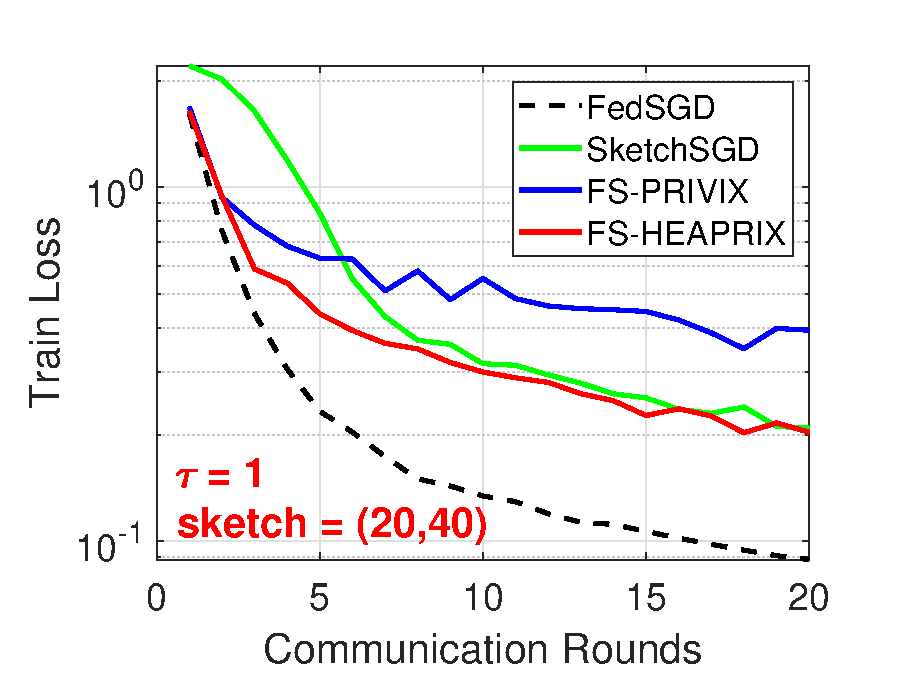
\includegraphics[width=3in]{MNIST_figures/local1_sketch20_iid1_train_loss.eps}
		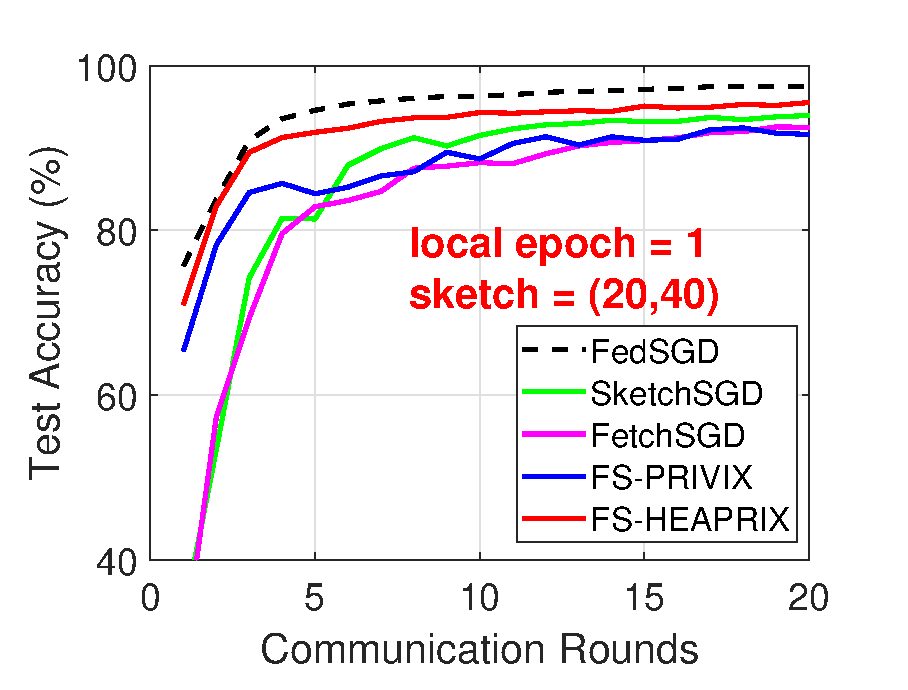
\includegraphics[width=3in]{MNIST_figures/local1_sketch20_iid1_test_acc.eps}
		}
		\mbox{
		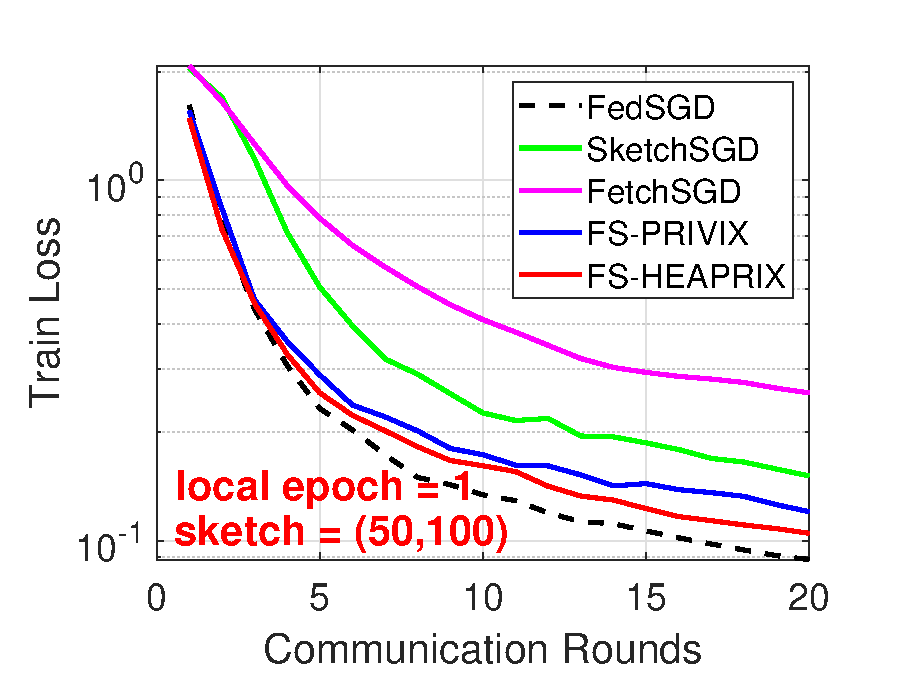
\includegraphics[width=3in]{MNIST_figures/local1_sketch50_iid1_train_loss.eps}
		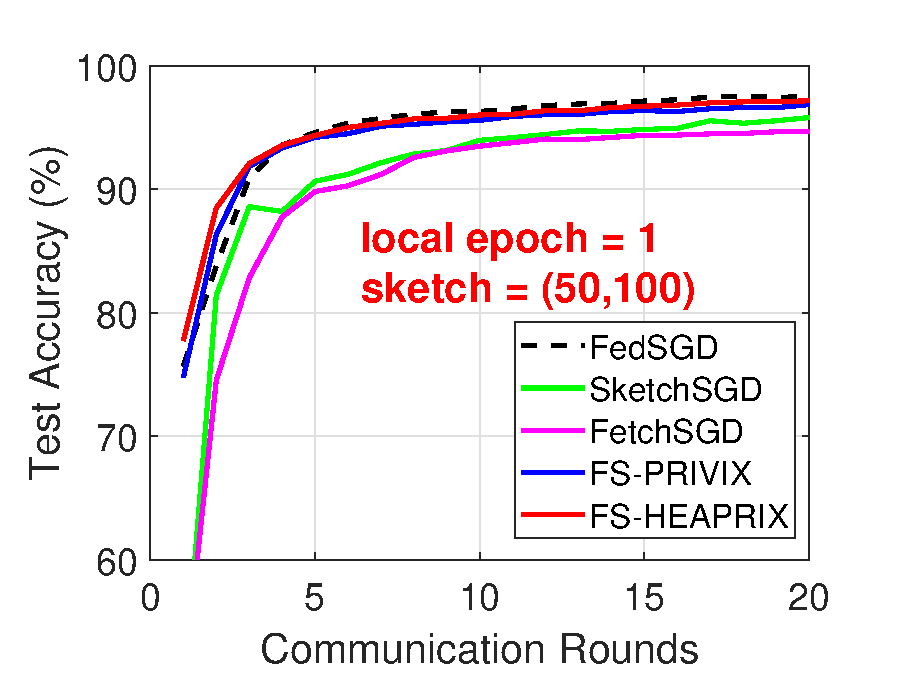
\includegraphics[width=3in]{MNIST_figures/local1_sketch50_iid1_test_acc.eps}
		}
	\end{center}
	\caption{The comparison of four algorithms on LeNet CNN architecture.}
    \label{fig:MNIST-tau1}
\end{figure}

\begin{figure}[h]
	\begin{center}
		\mbox{			    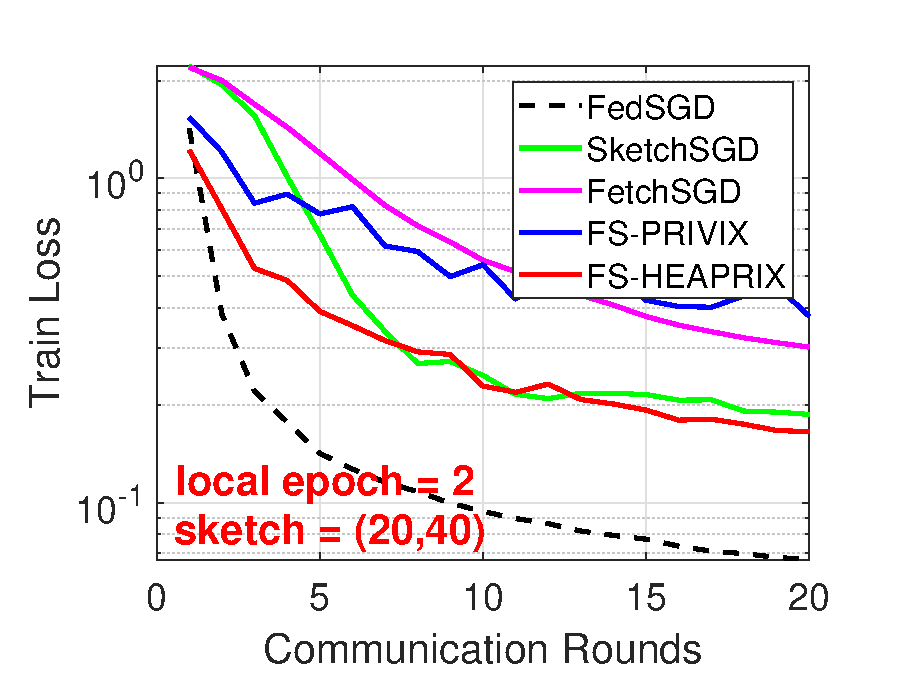
\includegraphics[width=1.6in]{MNIST_figures/local2_sketch20_iid1_train_loss.eps}
		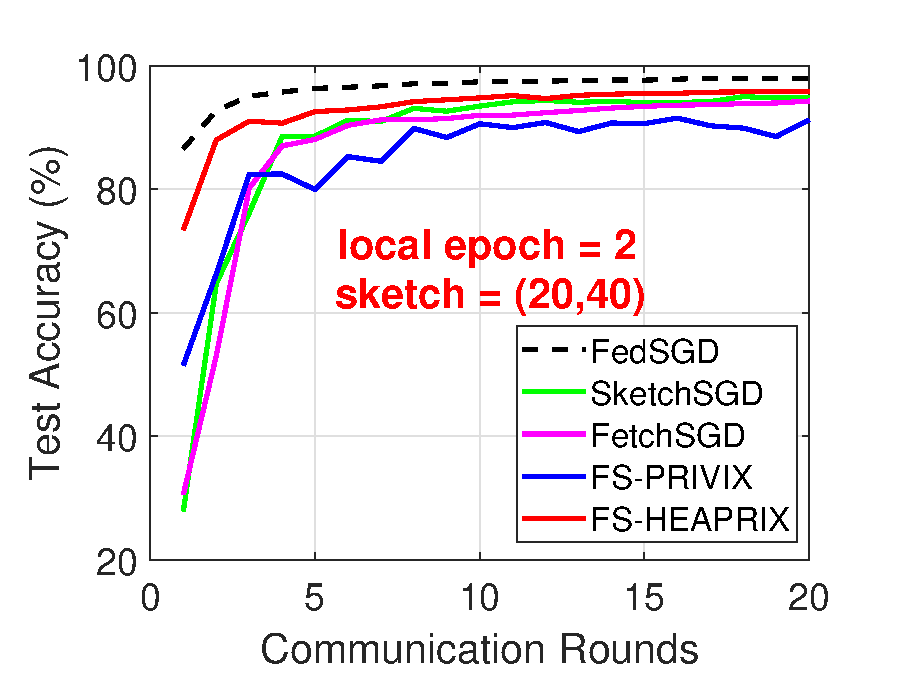
\includegraphics[width=1.6in]{MNIST_figures/local2_sketch20_iid1_test_acc.eps}
		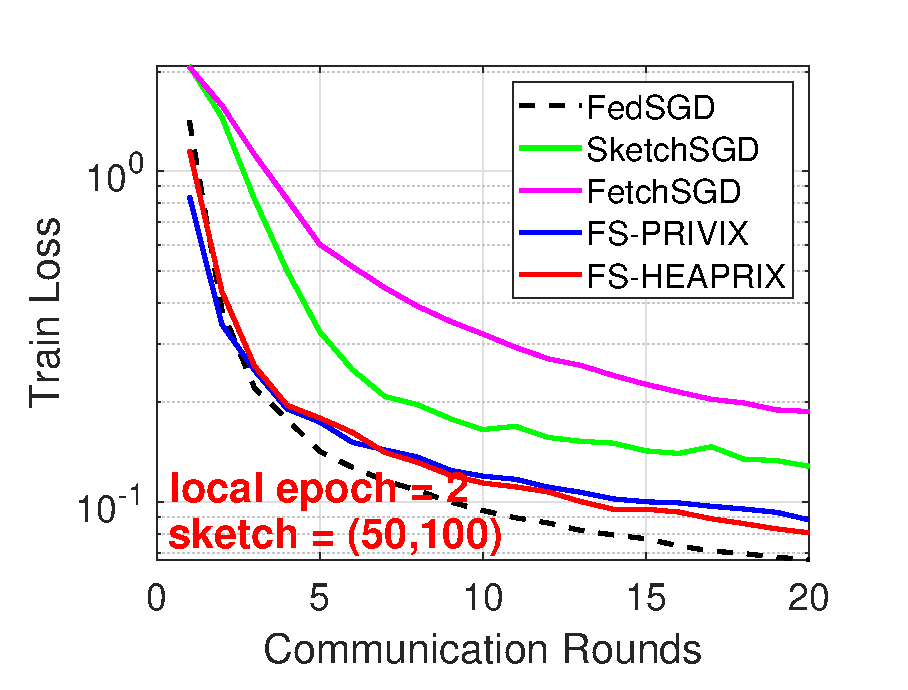
\includegraphics[width=1.6in]{MNIST_figures/local2_sketch50_iid1_train_loss.eps}
		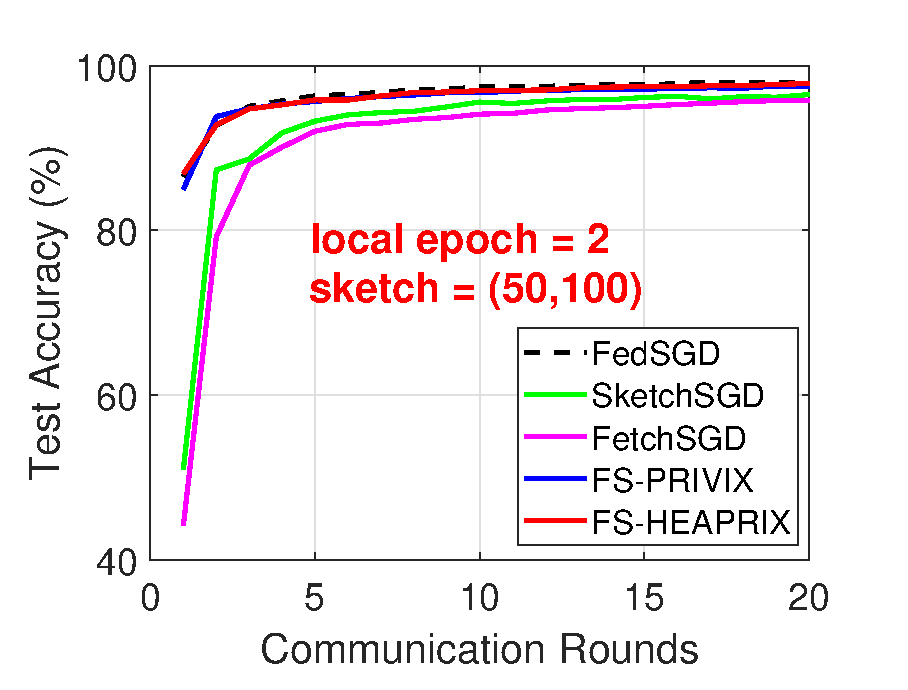
\includegraphics[width=1.6in]{MNIST_figures/local2_sketch50_iid1_test_acc.eps}
		}
		
		\mbox{			    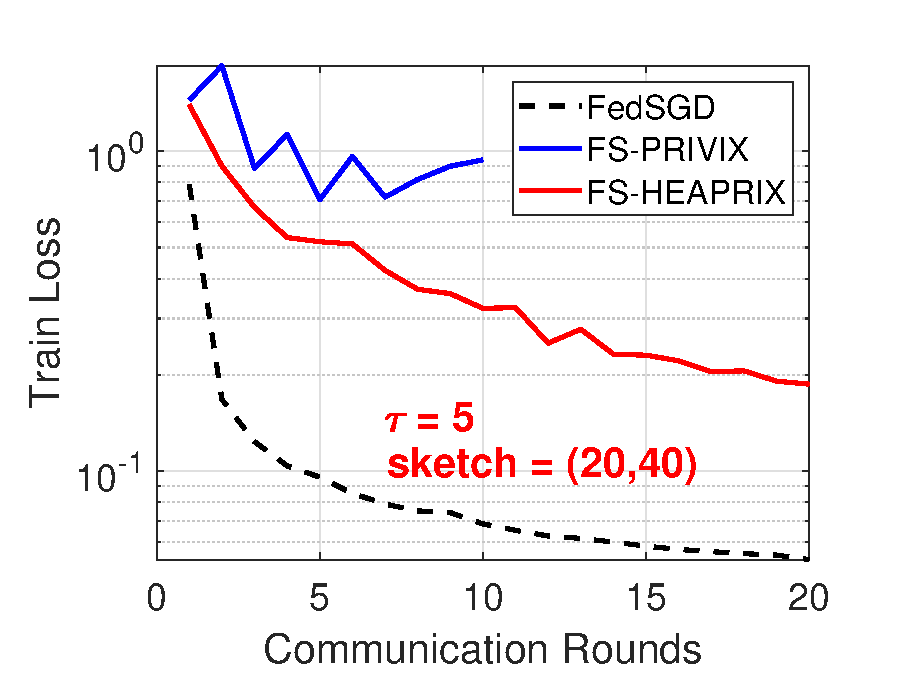
\includegraphics[width=1.6in]{MNIST_figures/local5_sketch20_iid1_train_loss.eps}
		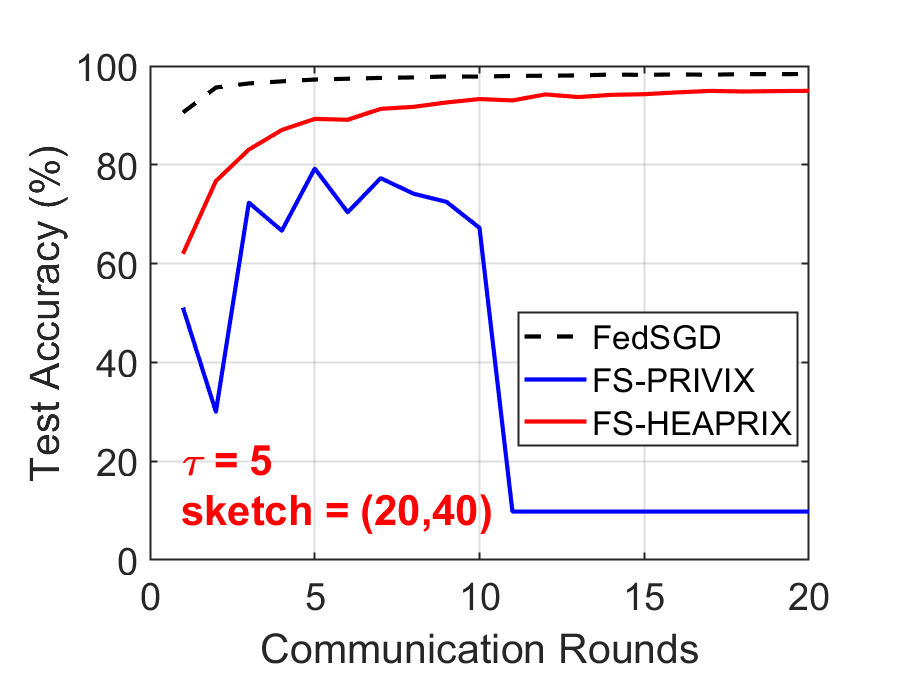
\includegraphics[width=1.6in]{MNIST_figures/local5_sketch20_iid1_test_acc.eps}
		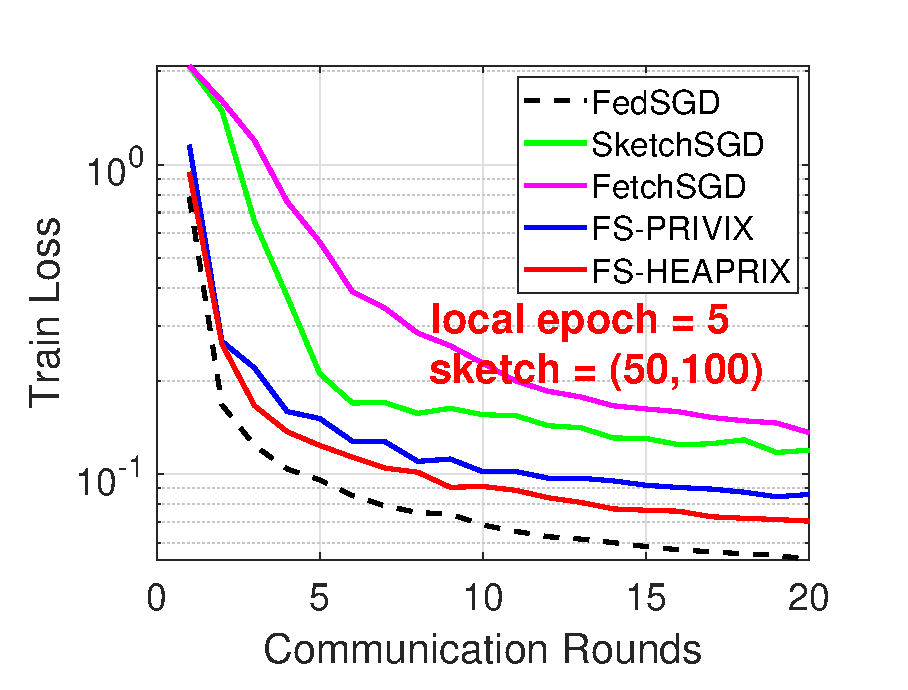
\includegraphics[width=1.6in]{MNIST_figures/local5_sketch50_iid1_train_loss.eps}
		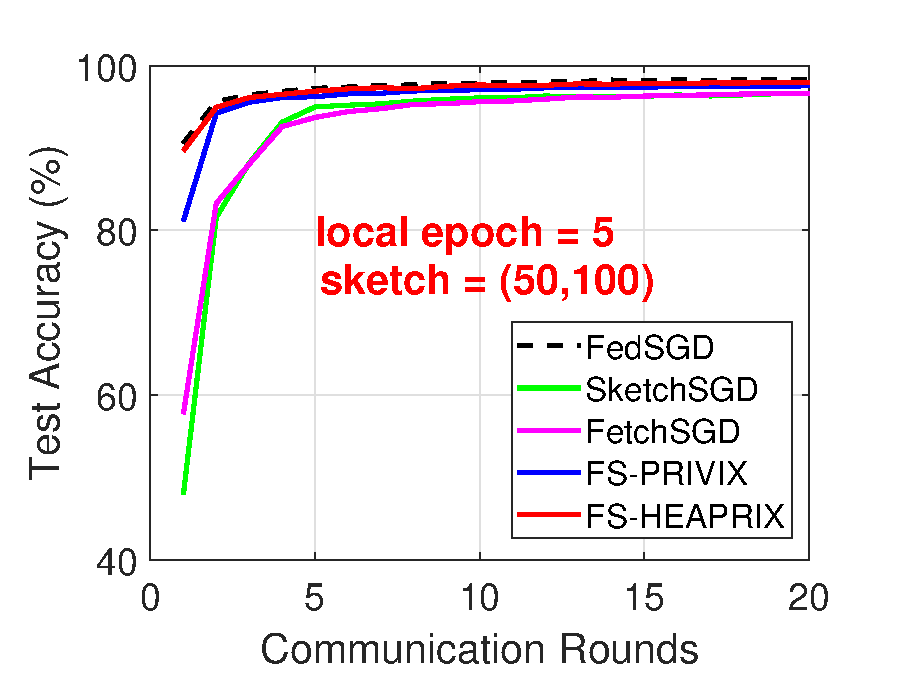
\includegraphics[width=1.6in]{MNIST_figures/local5_sketch50_iid1_test_acc.eps}
		}
	\end{center}
	\caption{Comparison of FedSGD, FS-PRIVIX and FS-HEAPRIX on LeNet CNN architecture, with number of local updates being 2 and 5.}
    \label{fig:MNIST-tau2,tau5}
\end{figure}


\textbf{Homogeneous case.} In Figure \ref{fig:MNIST-tau1} we provide the training loss and test accuracy of four algorithms with $\tau=1$ (since SketchSGD requires single local update per round). We also test different sizes of sketching matrix, $(t,k)=(20,40)$ and $(50,100)$. Note that these two choices of sketch size correspond to a $75\times$ and $12\times$ compression ratio, respectively. In general, as one would expect, higher compression ratio leads to worse learning performance. In both cases, FS-HEAPRIX performs the best in terms of both training objective and test accuracy. FS-PRIVIX is better when sketch size is large (i.e. when the estimation from sketches are more accurate), while SketchSGD performs better with small sketch size. 

The results for multiple local updates are given in Figure \ref{fig:MNIST-tau2,tau5}, where we set $\tau=2,5$. We see that FS-HEAPRIX is significantly better than FS-PRIVIX, either with small or large sketching matrix. In both cases, FS-HEAPRIX yields acceptable extra test error compared to FedSGD, especially taking the high compression ratio (e.g. $75\times$) into consideration. However, FS-PRIVIX performs poorly with small sketch size $(20,40)$, and even diverges with $\tau=5$. Another observation is that, the performance of FS-HEAPRIX improves with increasing number of local updates. That is, the proposed method is able to further reduce the communication cost by reducing the number of rounds required for communication. This is also consistent with our theoretical claims established in this paper.
\section{Conclusion}

In this paper, we introduced \texttt{FedSKETCH} and \texttt{FedSKETCHGATE} algorithms for homogeneous and heterogeneous data distribution setting respectively for Federated Learning wherein communication between server and devices is only performed using count sketch. 
Our algorithms, thus, provide communication-efficiency and privacy. 
We analyze the convergence error for \emph{non-convex}, \emph{\pl} and \emph{general convex} objective functions in the scope of Federated Optimization.  
We provide insightful numerical experiments showcasing the advantages of our FedSketch and FedSketchGATE methods over current federated optimization algorithm.

\clearpage
%%%%%%%%%%%%%%%%%%%%%%%%%%%%%%%%%%%%%%%%%%%%%%%%%%%%
\newpage
\bibliographystyle{IEEEtran}
\bibliography{references}
%%%%%%%%%%%%%%%%%%%%%%%%%%%%%%%%%%%%%%%%%%%%%%%%%%%%
\newpage
\appendix
\section{Appendix}
\section{Proof of main Theorems}
\subsection{Proof of Theorem~\ref{thm:homog_case}}

\subsection{Proof of Theorem~\ref{thm:hetreg_case}}
The following Lemma will be useful in our proof. 
\begin{lemma}
If you define $Q\triangleq3\sqrt[3]{\frac{ad^2}{2}}\sqrt{1+\sqrt{1+\frac{256 a}{27e^3d^4}}}$ and $$x\leq -\frac{1}{2}\sqrt{\frac{1}{3a}\left(Q-\frac{12a}{eQ}\right)}+\frac{1}{2}\sqrt{\frac{4}{eQ}-\frac{Q}{3a}+\frac{2d\sqrt{3}}{\sqrt{a}\sqrt{Q-\frac{12a}{e Q}}}}$$ then for positive constants $a,d,c\geq 0$, we have:
\begin{align}
    ax^{4}+dx-\frac{1}{e}\leq 0
\end{align}
\end{lemma}
\begin{proof}
We use the results in \cite{wiki:xxx} with $b=c=0$ and $p=0, q=\frac{d}{a}$. In this case, the only real valued root is 
\begin{align}
x&=-S+\frac{1}{2}\sqrt{-4S^2+\frac{d}{aS}},\:\text{and}\:S=\frac{1}{2}\sqrt{\frac{1}{3a}\left(Q-\frac{12a}{eQ}\right)}\nonumber\\
\implies x&=-\frac{1}{2}\sqrt{\frac{1}{3a}\left(Q-\frac{12a}{eQ}\right)}+\frac{1}{2}\sqrt{\frac{4}{eQ}-\frac{Q}{3a}+\frac{2d\sqrt{3}}{\sqrt{a}\sqrt{Q-\frac{12a}{e Q}}}} \nonumber\\
Q&=\sqrt[3]{\frac{{27a}{d^2}+\sqrt{\left({27a}{d^2}\right)^2+4\left(\frac{12a}{e}\right)^3}}{2}}=3\sqrt[3]{\frac{ad^2}{2}}\sqrt{1+\sqrt{1+\frac{256 a}{27e^3d^4}}}
\end{align} 
Therefore, we have with $Q=3\sqrt[3]{\frac{ad^2}{2}}\sqrt{1+\sqrt{1+\frac{256 a}{27e^3d^4}}}$:
\begin{align}
    x\leq -\frac{1}{2}\sqrt{\frac{1}{3a}\left(Q-\frac{12a}{eQ}\right)}+\frac{1}{2}\sqrt{\frac{4}{eQ}-\frac{Q}{3a}+\frac{2d\sqrt{3}}{\sqrt{a}\sqrt{Q-\frac{12a}{e Q}}}}
\end{align}
\end{proof}

Next, consider the following condition in~\cite{haddadpour2020federated}: 
\begin{align}
    \left(10\gamma^2L^4\tau^4\right)\eta^4+\left(L\gamma\tau\right)\eta-\frac{1}{q+1}\leq 0
\end{align}
where $a=10\gamma^2L^4\tau^4, d=L\gamma\tau$ and $e=q+1$, in this case 
\begin{align}
    Q=3\sqrt[3]{\frac{10}{2}}\gamma^{\frac{4}{3}} L^2\tau^2\underbrace{\sqrt{1+\sqrt{1+\frac{2560}{27\gamma^2(q+1)^3}}}}_{\triangleq C}=3\sqrt[3]{\frac{10}{2}}\gamma^{\frac{4}{3}} L^2\tau^2 C
\end{align}

Then we have:
\begin{align}
    x&\leq -\frac{1}{2}\sqrt{\frac{1}{3a}\left(Q-\frac{12a}{eQ}\right)}+\frac{1}{2}\sqrt{\frac{4}{eQ}-\frac{Q}{3a}+\frac{2d\sqrt{3}}{\sqrt{a}\sqrt{Q-\frac{12a}{e Q}}}}\nonumber\\
    &=-\frac{1}{2}\sqrt{\frac{3\sqrt[3]{\frac{10}{2}}\gamma^{\frac{4}{3}} L^2\tau^2 C}{30\gamma^2L^4\tau^4}-\frac{4}{(q+1)3\sqrt[3]{\frac{10}{2}}\gamma^{\frac{4}{3}} L^2\tau^2 C}}\nonumber\\
    &\quad+\frac{1}{2}\sqrt{\frac{4}{(q+1)3\sqrt[3]{\frac{10}{2}}\gamma^{\frac{4}{3}} L^2\tau^2 C}-\frac{3\sqrt[3]{\frac{10}{2}}\gamma^{\frac{4}{3}} L^2\tau^2 C}{30\gamma^2L^4\tau^4}+\frac{2L\gamma\tau\sqrt{3}}{\sqrt{10\gamma^2L^4\tau^4}\sqrt{3\sqrt[3]{\frac{10}{2}}\gamma^{\frac{4}{3}} L^2\tau^2 C-\frac{120 \gamma^2L^4\tau^4}{(q+1) 3\sqrt[3]{\frac{10}{2}}\gamma^{\frac{4}{3}} L^2\tau^2 C}}}}\nonumber\\
    &=\frac{1}{2L\tau\gamma^{\frac{1}{3}}}\Big(\sqrt{\frac{4}{(q+1)3\sqrt[3]{\frac{10}{2}}\gamma^{\frac{2}{3}} C}-\frac{\sqrt[3]{\frac{10}{2}} C}{10}+\frac{2\sqrt{3}}{\sqrt{10}\sqrt{3\sqrt[3]{\frac{10}{2}} C-\frac{40 }{(q+1)\gamma^{\frac{2}{3}} \sqrt[3]{\frac{10}{2}} C}}}}-\sqrt{\frac{\sqrt[3]{\frac{10}{2}} C}{10}-\frac{4}{(q+1)3\sqrt[3]{\frac{10}{2}}\gamma^{\frac{2}{3}} C}}\Big)\nonumber\\
\end{align}
%%%%%%%%%%%%%%%%%%%%%%%%%%%%%%%%%%%%%%%%%%%%%%%%
%%%%%%%%%%%%%%%%%%%%%%%%%%%%%%%%%%%%%%%%%%%%%%%%
\section{Convergence result for \texttt{FEDSKETCH} without memory}
From the $L$-smoothness gradient assumption on global objective, by using  $\underline{\mathbf{S}}^{(r)}=\tilde{\mathbf{g}}^{(r)}$ in inequality (\ref{eq:decent-smoothe}) we have:
\begin{align}
    f({\boldsymbol{x}}^{(r+1)})-f({\boldsymbol{x}}^{(r)})\leq -\gamma \big\langle\nabla f({\boldsymbol{x}}^{(r)}),\tilde{\mathbf{g}}^{(r)}\big\rangle+\frac{\gamma^2 L}{2}\|\tilde{\mathbf{g}}^{(r)}\|^2\label{eq:Lipschitz-c1}
\end{align}
We define the following:
\begin{align}
    \tilde{\mathbf{g}}_{\mathbf{S}}^{(r)}=\frac{\eta}{p}\sum_{j=1}^{p}\mathbf{S}\left[\sum_{c=0}^{\tau-1}\tilde{\mathbf{g}}_j^{(c,r)}\right]
\end{align}
Additionally, we define an auxiliary variable as 
\begin{align}
    \tilde{\mathbf{g}}^{(r)}=\frac{\eta}{p}\sum_{j=1}^{p}\left[\sum_{c=0}^{\tau-1}\tilde{\mathbf{g}}_j^{(c,r)}\right]
\end{align}
%%%%%%%%%%%%%%%%%%%%%%%%%%%%%%%%%%%%%%%%%%%%
By taking expectation on both sides of above inequality over sampling, we get:
\begin{align}
    \mathbb{E}\left[\mathbb{E}_\mathbf{S}\Big[f({\boldsymbol{x}}^{(r+1)})-f({\boldsymbol{x}}^{(r)})\Big]\right]&\leq -\gamma\mathbb{E}\left[\mathbb{E}_\mathbf{S}\left[ \big\langle\nabla f({\boldsymbol{x}}^{(r)}),\tilde{\mathbf{g}}_\mathbf{S}^{(r)}\big\rangle\right]\right]+\frac{\gamma^2 L}{2}\mathbb{E}\left[\mathbb{E}_\mathbf{S}\|\tilde{\mathbf{g}}_\mathbf{S}^{(r)}\|^2\right]\nonumber\\
    &=-\gamma\mathbb{E}\left[\mathbb{E}_\mathbf{S}\left[ \big\langle\nabla f({\boldsymbol{x}}^{(r)}),\tilde{\mathbf{g}}^{(r)}\big\rangle\right]\right]+\gamma\mathbb{E}\left[\mathbb{E}_\mathbf{S}\left[ \big\langle\nabla f({\boldsymbol{x}}^{(r)}),\tilde{\mathbf{g}}^{(r)}-\tilde{\mathbf{g}}_{\mathbf{S}}^{(r)}\big\rangle\right]\right]\nonumber\\
    &\qquad+\frac{\gamma^2 L}{2}\mathbb{E}\left[\mathbb{E}_\mathbf{S}\|\tilde{\mathbf{g}}_\mathbf{S}^{(r)}-\tilde{\mathbf{g}}^{(r)}+\tilde{\mathbf{g}}^{(r)}\|^2\right] \nonumber\\
    &\stackrel{(a)}{=}-\gamma\mathbb{E}\left[\mathbb{E}_\mathbf{S}\left[ \big\langle\nabla f({\boldsymbol{x}}^{(r)}),\tilde{\mathbf{g}}^{(r)}\big\rangle\right]\right]+\gamma\left[\mathbb{E}_\mathbf{S}\left[ \big\langle\nabla f({\boldsymbol{x}}^{(r)}),{\mathbf{g}}^{(r)}-{\mathbf{g}}_{\mathbf{S}}^{(r)}\big\rangle\right]\right]\nonumber\\
    &\qquad+\frac{\gamma^2 L}{2}\mathbb{E}\left[\mathbb{E}_\mathbf{S}\|\tilde{\mathbf{g}}_\mathbf{S}^{(r)}-\tilde{\mathbf{g}}^{(r)}+\tilde{\mathbf{g}}^{(r)}\|^2\right]\nonumber\\
    &\stackrel{(b)}{\leq}-\gamma\mathbb{E}\left[\mathbb{E}_\mathbf{S}\left[ \big\langle\nabla f({\boldsymbol{x}}^{(r)}),\tilde{\mathbf{g}}^{(r)}\big\rangle\right]\right]+\frac{\gamma}{2}\left[ \frac{1}{mL}\left\|\nabla f({\boldsymbol{x}}^{(r)})\right\|^2_2+mL\mathbb{E}_\mathbf{S}\left[\left\|{\mathbf{g}}^{(r)}-{\mathbf{g}}_{\mathbf{S}}^{(r)}\right\|^2_2\right]\right]\nonumber\\
    &\qquad+{\gamma^2 L}\mathbb{E}\left[\mathbb{E}_\mathbf{S}\left\|\tilde{\mathbf{g}}_\mathbf{S}^{(r)}-\tilde{\mathbf{g}}^{(r)}\right\|+\left\|\tilde{\mathbf{g}}^{(r)}\right\|^2\right] \nonumber\\
    &\stackrel{(c)}{\leq}-\gamma\mathbb{E}\left[ \big\langle\nabla f({\boldsymbol{x}}^{(r)}),\tilde{\mathbf{g}}^{(r)}\big\rangle\right]+\frac{\gamma}{2}\left[ \frac{1}{mL}\left\|\nabla f({\boldsymbol{x}}^{(r)})\right\|^2_2+mL\left(1-\frac{k}{d}\right)\left\|{\mathbf{g}}^{(r)}\right\|^2_2\right]\nonumber\\
    &\qquad+{\gamma^2 L}\mathbb{E}\left[\left(1-\frac{k}{d}\right)\left\|\tilde{\mathbf{g}}^{(r)}\right\|_2^2+\left\|\tilde{\mathbf{g}}^{(r)}\right\|_2^2\right]\nonumber\\
    &\stackrel{(d)}{=}-\gamma\underbrace{\mathbb{E}\left[ \big\langle\nabla f({\boldsymbol{x}}^{(r)}),\tilde{\mathbf{g}}^{(r)}\big\rangle\right]}_{(\mathrm{I})}+ \frac{\gamma}{2mL}\left\|\nabla f({\boldsymbol{x}}^{(r)})\right\|^2_2+\frac{mL\gamma}{2}\left(1-\frac{k}{d}\right)\underbrace{\left\|{\mathbf{g}}^{(r)}\right\|^2_2}_{(\mathrm{II})}\nonumber\\
    &\qquad+{\gamma^2 L}\left(2-\frac{k}{d}\right)\underbrace{\mathbb{E}\left[\left\|\tilde{\mathbf{g}}^{(r)}\right\|_2^2\right]}_{(\mathrm{III})}\label{eq:Lipschitz-c-gd-alt}
\end{align}
To bound term ($\mathrm{I}$) in Eq.~(\ref{eq:Lipschitz-c-gd-alt}) we use the combination of Lemmas~\ref{} and \ref{} we obtain:
\begin{align}
    -\gamma\mathbb{E}\left[ \big\langle\nabla f({\boldsymbol{x}}^{(r)}),\tilde{\mathbf{g}}^{(r)}\big\rangle\right]\leq \frac{\gamma}{2}\eta\frac{1}{p}\sum_{j=1}^p\sum_{c=0}^{\tau-1}\left[-\left\|\nabla f({\boldsymbol{x}}^{(r)})\right\|_2^2-\left\|\mathbf{g}_j^{(\ell,r)}\right\|_2^2+L^2\eta^2\sum_{\ell=0}^{\tau-1}\left[\tau\left\|{\mathbf{g}}_j^{(\ell,r)}\right\|_2^2+\sigma^2\right]\right]
\end{align}
Term $(\mathrm{II})$ can be bounded simply as follows:
\begin{align}
    \left\|{\mathbf{g}}^{(r)}\right\|^2_2&=\left\|\frac{\eta}{p}\sum_{j=1}^{p}\left[\sum_{c=0}^{\tau-1}{\mathbf{g}}_j^{(c,r)}\right]\right\|^2_2\nonumber\\
    &\leq\frac{\tau\eta^2}{p}\sum_{j=1}^{p}\sum_{c=0}^{\tau-1}\left\|\mathbf{g}_j^{(c,r)}\right\|^2_2
\end{align}

Next we bound term $(\mathrm{III})$ using the following lemma:
\begin{lemma}
\begin{align}
    \mathbb{E}\left[\left\|\tilde{\mathbf{g}}^{(r)}\right\|_2^2\right]\leq \frac{\eta^2\tau}{p}\sum_{j=1}^{p}\sum_{c=0}^{\tau-1}\left\|\mathbf{g}_j^{(c,r)}\right\|^2_2+\frac{\eta^2\tau}{p}\sigma^2
\end{align}
\end{lemma}
\begin{proof}
\begin{align}
    \mathbb{E}\left[\left\|\tilde{\mathbf{g}}^{(r)}\right\|_2^2\right]&=\mathbb{E}\left[\left\|\tilde{\mathbf{g}}^{(r)}-\mathbb{E}\left[\tilde{\mathbf{g}}^{(r)}\right]\right\|_2^2\right]+\left\|\mathbb{E}\left[\tilde{\mathbf{g}}^{(r)}\right]\right\|^2_2\nonumber\\
    &= \mathbb{E}\left[\left\|\tilde{\mathbf{g}}^{(r)}-{\mathbf{g}}^{(r)}\right\|_2^2\right]+\left\|{\mathbf{g}}^{(r)}\right\|^2_2\nonumber\\
    &= \mathbb{E}\left[\left\|\frac{\eta}{p}\sum_{j=1}^{p}\left[\sum_{c=0}^{\tau-1}\tilde{\mathbf{g}}_j^{(c,r)}\right]-\frac{\eta}{p}\sum_{j=1}^{p}\left[\sum_{c=0}^{\tau-1}\mathbf{g}_j^{(c,r)}\right]\right\|_2^2\right]+\left\|\frac{\eta}{p}\sum_{j=1}^{p}\left[\sum_{c=0}^{\tau-1}\mathbf{g}_j^{(c,r)}\right]\right\|^2_2\nonumber\\
&=\frac{\eta^2}{p^2}\sum_{j=1}^{p}\sum_{c=0}^{\tau-1}\mathbb{E}\left[\left\|\tilde{\mathbf{g}}_j^{(c,r)}-\mathbf{g}_j^{(c,r)}\right\|_2^2\right]+\left\|\frac{\eta}{p}\sum_{j=1}^{p}\left[\sum_{c=0}^{\tau-1}\mathbf{g}_j^{(c,r)}\right]\right\|^2_2 \nonumber\\
&\leq \frac{\eta^2}{p^2}\sum_{j=1}^{p}\sum_{c=0}^{\tau-1}\mathbb{E}\left[\left\|\tilde{\mathbf{g}}_j^{(c,r)}-\mathbf{g}_j^{(c,r)}\right\|_2^2\right]+\frac{\eta^2\tau}{p}\sum_{j=1}^{p}\sum_{c=0}^{\tau-1}\left\|\mathbf{g}_j^{(c,r)}\right\|^2_2\nonumber\\
&\leq \frac{\eta^2}{p^2}\sum_{j=1}^{p}\sum_{c=0}^{\tau-1}\sigma^2+\frac{\eta^2\tau}{p}\sum_{j=1}^{p}\sum_{c=0}^{\tau-1}\left\|\mathbf{g}_j^{(c,r)}\right\|^2_2\nonumber\\
&=\frac{\eta^2\tau}{p}\sum_{j=1}^{p}\sum_{c=0}^{\tau-1}\left\|\mathbf{g}_j^{(c,r)}\right\|^2_2+\frac{\eta^2\tau}{p}\sigma^2
\end{align}
\end{proof}
Next, we put all the pieces together as follows:
\begin{align}
    \mathbb{E}\left[\mathbb{E}_\mathbf{S}\Big[f({\boldsymbol{x}}^{(r+1)})-f({\boldsymbol{x}}^{(r)})\Big]\right]&\leq \frac{\gamma}{2}\eta\frac{1}{p}\sum_{j=1}^p\sum_{\ell=0}^{\tau-1}\left[-\left\|\nabla f({\boldsymbol{x}}^{(r)})\right\|_2^2-\left\|\mathbf{g}_j^{(\ell,r)}\right\|_2^2+L^2\eta^2\sum_{\ell=0}^{\tau-1}\left[\tau\left\|{\mathbf{g}}_j^{(\ell,r)}\right\|_2^2+\sigma^2\right]\right]\nonumber\\
    &\quad+ \frac{\gamma}{2mL}\left\|\nabla f({\boldsymbol{x}}^{(r)})\right\|^2_2+\frac{mL\gamma}{2}\left(1-\frac{k}{d}\right)\frac{\tau\eta^2}{p}\sum_{j=1}^{p}\sum_{\ell=0}^{\tau-1}\left\|\mathbf{g}_j^{(\ell,r)}\right\|^2_2\nonumber\\
    &\quad+\gamma^2 L\left(2-\frac{k}{d}\right)\left[\frac{\eta^2\tau}{p}\sum_{j=1}^{p}\sum_{c=0}^{\tau-1}\left\|\mathbf{g}_j^{(\ell,r)}\right\|^2_2+\frac{\eta^2\tau}{p}\sigma^2\right]\nonumber\\
    &=-\frac{\tau\eta\gamma}{2}\left\|\nabla f({\boldsymbol{x}}^{(r)})\right\|_2^2+\frac{\gamma}{2}\eta\frac{1}{p}\sum_{j=1}^p\sum_{\ell=0}^{\tau-1}\left[-\left\|\mathbf{g}_j^{(\ell,r)}\right\|_2^2+L^2\eta^2\tau^2\left\|{\mathbf{g}}_j^{(\ell,r)}\right\|_2^2\right]+\frac{\gamma\eta^3L^2\tau^2}{2}\sigma^2\nonumber\\
    &\quad+ \frac{\gamma}{2mL}\left\|\nabla f({\boldsymbol{x}}^{(r)})\right\|^2_2+\frac{mL\gamma}{2}\left(1-\frac{k}{d}\right)\frac{\tau\eta^2}{p}\sum_{j=1}^{p}\sum_{\ell=0}^{\tau-1}\left\|\mathbf{g}_j^{(\ell,r)}\right\|^2_2\nonumber\\
    &\quad+\gamma^2 L\left(2-\frac{k}{d}\right)\frac{\eta^2\tau}{p}\sum_{j=1}^{p}\sum_{\ell=0}^{\tau-1}\left\|\mathbf{g}_j^{(\ell,r)}\right\|^2_2+\gamma^2 L\left(2-\frac{k}{d}\right)\frac{\eta^2\tau}{p}\sigma^2\nonumber\\
    &=-\left(\frac{\tau\eta\gamma}{2}-\frac{\gamma}{2mL}\right)\left\|\nabla f({\boldsymbol{x}}^{(r)})\right\|_2^2\nonumber\\
    &\quad-\left(\frac{\eta\gamma}{2}-\frac{\eta\gamma}{2}\left(L^2\eta^2\tau^2\right)-\frac{mL\eta\gamma}{2}\left(1-\frac{k}{d}\right)\tau\eta-\gamma^2 L\eta^2\tau\left(2-\frac{k}{d}\right)\right)\frac{1}{p}\sum_{j=1}^{p}\sum_{\ell=0}^{\tau-1}\left\|\mathbf{g}_j^{(\ell,r)}\right\|^2_2\nonumber\\
    &\quad+\frac{\gamma\eta^3L^2\tau^2}{2}\sigma^2+\gamma^2 L\left(2-\frac{k}{d}\right)\frac{\eta^2\tau}{p}\sigma^2\nonumber\\
    &\stackrel{(a)}{\leq}-\left(\frac{\tau\eta\gamma}{2}-\frac{\gamma}{2mL}\right)\left\|\nabla f({\boldsymbol{x}}^{(r)})\right\|_2^2+\frac{\gamma\eta^3L^2\tau^2}{2}\sigma^2+\tau\eta^2\gamma^2 L\left(2-\frac{k}{d}\right)\frac{\sigma^2}{p}\label{eq:ncvx-mid-step}
\end{align}
where (a) follows from the learning rate choices of 
\begin{align}
    \frac{\eta\gamma}{2}-\frac{\eta\gamma}{2}\left(L^2\eta^2\tau^2\right)-\frac{mL\eta\gamma}{2}\left(1-\frac{k}{d}\right)\tau\eta-\gamma^2 L\eta^2\tau\left(2-\frac{k}{d}\right)\geq 0
\end{align}
which can be simplified further as follows:
\begin{align}
    1-L^2\eta^2\tau^2-mL\tau\eta\left(1-\frac{k}{d}\right)-2\gamma L\eta\tau\left(2-\frac{k}{d}\right)\geq 0
\end{align}
Then using Eq.~(\ref{eq:ncvx-mid-step}) we obtain:
\begin{align}
  \frac{\tau\gamma}{2} \left({\eta}-\frac{1}{\tau mL}\right)\left\|\nabla f({\boldsymbol{x}}^{(r)})\right\|_2^2\leq \mathbb{E}\left[\mathbb{E}_\mathbf{S}\Big[f({\boldsymbol{x}}^{(r+1)})-f({\boldsymbol{x}}^{(r)})\Big]\right]+\tau\eta^2\gamma^2 L\left(2-\frac{k}{d}\right)\frac{\sigma^2}{p}+\frac{\gamma\eta^3L^2\tau^2}{2}\sigma^2
\end{align}
which leads to the following bound:
\begin{align}
     \left\|\nabla f({\boldsymbol{x}}^{(r)})\right\|_2^2\leq \frac{2 \mathbb{E}\left[\mathbb{E}_\mathbf{S}\Big[f({\boldsymbol{x}}^{(r+1)})-f({\boldsymbol{x}}^{(r)})\Big]\right]}{\tau \gamma \left({\eta}-\frac{1}{\tau mL}\right)}+\frac{2\eta^2\gamma L\left(2-\frac{k}{d}\right)\frac{\sigma^2}{p}}{ \left({\eta}-\frac{1}{\tau mL}\right)}+\frac{\eta^3L^2\tau}{\left({\eta}-\frac{1}{\tau mL}\right)}\sigma^2 
\end{align}
Now averaging over $r$ communication rounds we achieve:
\begin{align}
    \frac{1}{R}\sum_{r=0}^{R-1}\left\|\nabla f({\boldsymbol{x}}^{(r)})\right\|_2^2\leq \frac{2 \mathbb{E}\left[\mathbb{E}_\mathbf{S}\Big[f({\boldsymbol{x}}^{(0)})-f({\boldsymbol{x}}^{(*)})\Big]\right]}{R\tau \gamma \left({\eta}-\frac{1}{\tau mL}\right)}+\frac{2\eta^2\gamma L\left(2-\frac{k}{d}\right)\frac{\sigma^2}{p}}{ \left({\eta}-\frac{1}{\tau mL}\right)}+\frac{\eta^3L^2\tau}{\left({\eta}-\frac{1}{\tau mL}\right)}\sigma^2 
\end{align}
We note that for this case we have the following conditions over learning rate:
\begin{align}
    L^2\eta^2\tau^2+mL\tau\eta\left(1-\frac{k}{d}\right)+2\gamma L\eta\tau\left(2-\frac{k}{d}\right)\leq 1,\:\eta> \frac{1}{mL\tau},
\end{align}

\subsection{Proof of Theorem~\ref{thm:pl-iid}}
From Eq.~(\ref{eq:ncvx-mid-step}) under condition with:
\begin{align}
       L^2\eta^2\tau^2+mL\tau\eta\left(1-\frac{k}{d}\right)+2\gamma L\eta\tau\left(2-\frac{k}{d}\right)\leq 1, \label{eq:step_size_cnd_mmr}
\end{align}
we obtain:
\begin{align}
         \mathbb{E}\left[f({\boldsymbol{w}}^{(r+1)})-f({\boldsymbol{w}}^{(r)})\right]&\leq -\left(\frac{\tau\eta\gamma}{2}-\frac{\gamma}{2mL}\right)\left\|\nabla f({\boldsymbol{x}}^{(r)})\right\|_2^2+\frac{\gamma\eta^3L^2\tau^2}{2}\sigma^2+\tau\eta^2\gamma^2 L\left(2-\frac{k}{d}\right)\frac{\sigma^2}{p}\nonumber\\
         &\stackrel{(PL)}{\leq} -\left({\tau\mu\eta\gamma}-\frac{\mu\gamma}{mL}\right)\left[f({\boldsymbol{w}}^{(r)})-f({\boldsymbol{w}}^{(*)})\right]+\frac{\gamma\eta^3L^2\tau^2}{2}\sigma^2+\tau\eta^2\gamma^2 L\left(2-\frac{k}{d}\right)\frac{\sigma^2}{p} 
\end{align}
which leads to the following bound:
\begin{align}
            \mathbb{E}\Big[f({\boldsymbol{w}}^{(r+1)})-f({\boldsymbol{w}}^{(*)})\Big]&\leq \left(1-\eta\mu\gamma{\tau}+\frac{\mu\gamma}{mL}\right) \Big[f({\boldsymbol{w}}^{(r)})-f({\boldsymbol{w}}^{(*)})\Big]+\frac{\gamma\eta^3L^2\tau^2}{2}\sigma^2+\tau\eta^2\gamma^2 L\left(2-\frac{k}{d}\right)\frac{\sigma^2}{p} 
\end{align}
which leads to the following bound by setting $\Delta\triangleq1-\eta\mu\gamma{\tau}+\frac{\mu\gamma}{mL}=1-\mu\gamma\tau\left(\eta-\frac{1}{mL\tau}\right)$:
\begin{align}
            \mathbb{E}\Big[f({\boldsymbol{w}}^{(R)})-f({\boldsymbol{w}}^{(*)})\Big]&\leq \Delta^R \Big[f({\boldsymbol{w}}^{(0)})-f({\boldsymbol{w}}^{(*)})\Big]+\frac{1-\Delta^R}{1-\Delta}\left(\frac{\gamma\eta^3L^2\tau^2}{2}\sigma^2+\tau\eta^2\gamma^2 L\left(2-\frac{k}{d}\right)\frac{\sigma^2}{p} \right)\nonumber\\
            &\leq \Delta^R \Big[f({\boldsymbol{w}}^{(0)})-f({\boldsymbol{w}}^{(*)})\Big]+\frac{1}{1-\Delta}\left(\frac{\gamma\eta^3L^2\tau^2}{2}\sigma^2+\tau\eta^2\gamma^2 L\left(2-\frac{k}{d}\right)\frac{\sigma^2}{p} \right)\nonumber\\
            &={\left(1-\mu\gamma\tau\left(\eta-\frac{1}{mL\tau}\right)\right)}^R \Big[f({\boldsymbol{w}}^{(0)})-f({\boldsymbol{w}}^{(*)})\Big]+\frac{\left(\frac{\gamma\eta^3L^2\tau^2}{2}\sigma^2+\tau\eta^2\gamma^2 L\left(2-\frac{k}{d}\right)\frac{\sigma^2}{p} \right)}{\mu\gamma\tau\left(\eta-\frac{1}{m L\tau}\right)}\nonumber\\
            &\leq \exp{-\left(\mu\gamma\tau\left(\eta-\frac{1}{m L\tau}\right)R\right)}\Big[f({\boldsymbol{w}}^{(0)})-f({\boldsymbol{w}}^{(*)})\Big]+\frac{\left(\frac{\gamma\eta^3L^2\tau}{2}\sigma^2+\eta^2\gamma^2 L\left(2-\frac{k}{d}\right)\frac{\sigma^2}{p} \right)}{\mu\gamma\left(\eta-\frac{1}{mL\tau}\right)}
\end{align}
Then for the choice of $\eta=\frac{n}{mL\tau}$, for $m>n>1$, we obtain:


\begin{align}
                \mathbb{E}\Big[f({\boldsymbol{w}}^{(R)})-f({\boldsymbol{w}}^{(*)})\Big]&\leq \exp{-\left(\frac{\gamma\left(n-1\right) R}{m\kappa}\right) }\Big[f({\boldsymbol{w}}^{(0)})-f({\boldsymbol{w}}^{(*)})\Big]+\frac{\left(\frac{\gamma n^3L^2\tau}{2m^3L^3\tau^3}\sigma^2+\frac{n^2}{m^2L^2\tau^2}\gamma^2 L\left(2-\frac{k}{d}\right)\frac{\sigma^2}{p} \right)}{\mu\gamma\left(\frac{n-1}{mL\tau}\right)}\nonumber\\
                &=\exp{-\left(\frac{\gamma\left(n-1\right) R}{m\kappa}\right) }\Big[f({\boldsymbol{w}}^{(0)})-f({\boldsymbol{w}}^{(*)})\Big]+\frac{\left(\frac{ n^3}{2m^2}+\frac{n^2}{m}\gamma L\left(2-\frac{k}{d}\right)\frac{1}{p} \right)}{\mu\tau\left(n-1\right)}\sigma^2
\end{align}

We note that regarding condition in Eq.~(\ref{eq:step_size_cnd_mmr}), if we let $\eta=\frac{n}{m L\tau}$ for $m>n>1$, we need to satisfy the following condition:
\begin{align}
    \frac{n^2}{m^2}+n\left(1-\frac{k}{d}\right)+\frac{2n\gamma\left(1-\frac{k}{d}\right)}{m}\leq 1
\end{align}
Now if you let $\gamma=\frac{m}{2}$, we need to impose the following condition over $k$ and $d$ as follows:
\begin{align}
    n\left(1-\frac{k}{d}\right)\leq \frac{1}{3}\implies d\left(1-\frac{1}{3n}\right)\leq k\leq d
\end{align}
\todo{Will fix these later!}





\end{document}
